% -*- Mode:TeX -*-

%% IMPORTANT: The official thesis specifications are available at:
%%            http://libraries.mit.edu/archives/thesis-specs/
%%
%%            Please verify your thesis' formatting and copyright
%%            assignment before submission. If you notice any
%%            discrepancies between these templates and the
%%            MIT Libraries' specs, please let us know
%%            by e-mailing thesis@mit.edu


%% The documentclass options along with the pagestyle can be used to generate
%% a technical report, a draft copy, or a regular thesis. You may need to
%% re-specify the pagestyle after you \include cover.tex. For more
%% information, see the first few lines of mitthesis.cls.

%\documentclass[12pt,vi,twoside]{mitthesis}
%%
%%  If you want your thesis copyright to you instead of MIT, use the
%%  ``vi'' option, as above.
%%
%\documentclass[12pt,twoside,leftblank]{mitthesis}
%%
%% If you want blank pages before new chapters to be labelled ``This
%% Page Intentionally Left Blank'', use the ``leftblank'' option, as
%% above.

\documentclass[12pt,oneside]{mitthesis}
\usepackage{lgrind}
%% These have been added at the request of the MIT Libraries, because
%% some PDF conversions mess up the ligatures.  -LB, 1/22/2014
\usepackage{cmap}
\usepackage{verbatim}
\usepackage{enumitem}
\usepackage{amsmath}
\usepackage{booktabs}
\usepackage[bottom]{footmisc}
\usepackage{graphicx}
\usepackage{array}
\usepackage{float}
\usepackage{ragged2e}
\usepackage{makecell}
\usepackage{adjustbox}
\usepackage{threeparttablex}
\usepackage{caption}
\usepackage{multicol}
\usepackage[natbib,style=authoryear]{biblatex}
\bibliography{Bibliography.bib}
\usepackage[T1]{fontenc}
\pagestyle{plain}
\graphicspath{{C:/repos/learn-doing/thesis/figures/}{C:/repos/learn-doing/R/Output/}}
%% This bit allows you to either specify only the files which you wish to
%% process, or `all' to process all files which you \include.
%% Krishna Sethuraman (1990).

%\typein [\files]{Enter file names to process, (chap1,chap2 ...), or `all' to process all files:}
\def\all{all}
\ifx\files\all \typeout{Including all files.} \else %\typeout{Including only \files.} \includeonly{\files} \fi
\usepackage{titlesec}



%\degree{Master of Arts in Social Science, Economics Concentration}
%\degreeword{degree}

\begin{document}

\begin{titlepage}
   \begin{center}

  \vspace*{3cm}

{\LARGE THE UNIVERSITY OF CHICAGO}

\vspace*{1.5cm}

{\Huge Learning by Doing in Public Construction Contracts}

\vspace*{1.5cm}

{\LARGE By}

\vspace*{1.5cm}

{\Huge Maximiliano José González Busse}

\vspace*{1.5cm}

{\LARGE August 2021}

\vspace*{1.5cm}

{\large A paper submitted in partial fulfillment of the requirements of the Master of Arts degree in the Master of Arts Program in the Social Sciences, Economics Concentration}

\vspace*{2.5cm}
   \end{center}

{\large Faculty Advisor: Casey B. Mulligan}

\end{titlepage}

\setcounter{tocdepth}{1}




\centering
\textbf{Abstract}
\justify
\footnotesize
Using 43,000 public construction contracts in Chile procured via competitive calls for proposals, I study the effect of firm experience on the likelihood of winning a contract in the future. To address endogeneity of experience (better firms tend to win more contracts in the past and in the future), I instrument firm experience with the number of past contracts won in closely contested auctions, where close auctions are defined as either i) having close monetary bids and price as an important awarding factor, or ii) involving closely ranked firms (via a multiplayer Elo algorithm) . The IV estimates indicate that firm's experience increases the proportion of contracts won by seven percentage points (roughly a third of the winning rate of firms with no experience). I investigate possible mechanisms that could explain this increase in market success by studying improvements along i) cost measures and ii) quality variables. I find that experienced firms submit bids which are three percentage points lower than firms with no experience. Additionally, experienced firms increase in ten percentage points the approval rate of their proposals in the first stage of the awarding process. I discuss the magnitude of the findings and possible implications for public auction design.

\small
%\tableofcontents
%\thispagestyle{empty}
%\listoffigures
%\listoftables
\normalsize
\justify
%% -*-latex-*-
%
% For questions, comments, concerns or complaints:
% thesis@mit.edu
%
%
% $Log: cover.tex,v $
% Revision 1.9  2019/08/06 14:18:15  cmalin
% Replaced sample content with non-specific text.
%
% Revision 1.8  2008/05/13 15:02:15  jdreed
% Degree month is June, not May.  Added note about prevdegrees.
% Arthur Smith's title updated
%
% Revision 1.7  2001/02/08 18:53:16  boojum
% changed some \newpages to \cleardoublepages
%
% Revision 1.6  1999/10/21 14:49:31  boojum
% changed comment referring to documentstyle
%
% Revision 1.5  1999/10/21 14:39:04  boojum
% *** empty log message ***
%
% Revision 1.4  1997/04/18  17:54:10  othomas
% added page numbers on abstract and cover, and made 1 abstract
% page the default rather than 2.  (anne hunter tells me this
% is the new institute standard.)
%
% Revision 1.4  1997/04/18  17:54:10  othomas
% added page numbers on abstract and cover, and made 1 abstract
% page the default rather than 2.  (anne hunter tells me this
% is the new institute standard.)
%
% Revision 1.3  93/05/17  17:06:29  starflt
% Added acknowledgements section (suggested by tompalka)
%
% Revision 1.2  92/04/22  13:13:13  epeisach
% Fixes for 1991 course 6 requirements
% Phrase "and to grant others the right to do so" has been added to
% permission clause
% Second copy of abstract is not counted as separate pages so numbering works
% out
%
% Revision 1.1  92/04/22  13:08:20  epeisach

% NOTE:
% These templates make an effort to conform to the MIT Thesis specifications,
% however the specifications can change. We recommend that you verify the
% layout of your title page with your thesis advisor and/or the MIT
% Libraries before printing your final copy.
\title{Master of Arts Thesis}

\author{Maximiliano  Gonzalez}
% If you wish to list your previous degrees on the cover page, use the
% previous degrees command:
%       \prevdegrees{A.A., Harvard University (1985)}
% You can use the \\ command to list multiple previous degrees
%       \prevdegrees{B.S., University of California (1978) \\
%                    S.M., Massachusetts Institute of Technology (1981)}
\department{Kenneth C. Griffin Department of Economics}

% If the thesis is for two degrees simultaneously, list them both
% separated by \and like this:
% \degree{Doctor of Philosophy \and Master of Science}
\degree{Master of Arts in Social Sciences, Economics Concentration}

% As of the 2007-08 academic year, valid degree months are September,
% February, or June.  The default is June.
\degreemonth{April}
\degreeyear{2021}
\thesisdate{April 18, 2021}

%% By default, the thesis will be copyrighted to MIT.  If you need to copyright
%% the thesis to yourself, just specify the `vi' documentclass option.  If for
%% some reason you want to exactly specify the copyright notice text, you can
%% use the \copyrightnoticetext command.
%\copyrightnoticetext{\copyright IBM, 1990.  Do not open till Xmas.}

% If there is more than one supervisor, use the \supervisor command
% once for each.
\supervisor{William J. Supervisor}{Associate Professor}

% This is the department committee chairman, not the thesis committee
% chairman.  You should replace this with your Department's Committee
% Chairman.
\chairman{Arthur C. Chairman}{Chairman, Department Committee on Graduate Theses}

% Make the titlepage based on the above information.  If you need
% something special and can't use the standard form, you can specify
% the exact text of the titlepage yourself.  Put it in a titlepage
% environment and leave blank lines where you want vertical space.
% The spaces will be adjusted to fill the entire page.  The dotted
% lines for the signatures are made with the \signature command.
\maketitle

% The abstractpage environment sets up everything on the page except
% the text itself.  The title and other header material are put at the

% top of the page, and the supervisors are listed at the bottom.  A
% new page is begun both before and after.  Of course, an abstract may
% be more than one page itself.  If you need more control over the
% format of the page, you can use the abstract environment, which puts
% the word "Abstract" at the beginning and single spaces its text.

%% You can either \input (*not* \include) your abstract file, or you can put
%% the text of the abstract directly between the \begin{abstractpage} and
%% \end{abstractpage} commands.

% First copy: start a new page, and save the page number.
\cleardoublepage
% Uncomment the next line if you do NOT want a page number on your
% abstract and acknowledgments pages.
% \pagestyle{empty}
\setcounter{savepage}{\thepage}
\begin{abstractpage}


\centering
\textbf{Abstract}
\justify
\footnotesize
Using 43,000 public construction contracts in Chile procured via competitive calls for proposals, I study the effect of firm experience on the likelihood of winning a contract in the future. To address endogeneity of experience (better firms tend to win more contracts in the past and in the future), I instrument firm experience with the number of past contracts won in closely contested auctions, where close auctions are defined as either i) having close monetary bids and price as an important awarding factor, or ii) involving closely ranked firms (via a multiplayer Elo algorithm) . The IV estimates indicate that firm's experience increases the proportion of contracts won by seven percentage points (roughly a third of the winning rate of firms with no experience). I investigate possible mechanisms that could explain this increase in market success by studying improvements along i) cost measures and ii) quality variables. I find that experienced firms submit bids which are three percentage points lower than firms with no experience. Additionally, experienced firms increase in ten percentage points the approval rate of their proposals in the first stage of the awarding process. I discuss the magnitude of the findings and possible implications for public auction design.

\end{abstractpage}

% Additional copy: start a new page, and reset the page number.  This way,
% the second copy of the abstract is not counted as separate pages.
% Uncomment the next 6 lines if you need two copies of the abstract
% page.
% \setcounter{page}{\thesavepage}
% \begin{abstractpage}
% 

\centering
\textbf{Abstract}
\justify
\footnotesize
Using 43,000 public construction contracts in Chile procured via competitive calls for proposals, I study the effect of firm experience on the likelihood of winning a contract in the future. To address endogeneity of experience (better firms tend to win more contracts in the past and in the future), I instrument firm experience with the number of past contracts won in closely contested auctions, where close auctions are defined as either i) having close monetary bids and price as an important awarding factor, or ii) involving closely ranked firms (via a multiplayer Elo algorithm) . The IV estimates indicate that firm's experience increases the proportion of contracts won by seven percentage points (roughly a third of the winning rate of firms with no experience). I investigate possible mechanisms that could explain this increase in market success by studying improvements along i) cost measures and ii) quality variables. I find that experienced firms submit bids which are three percentage points lower than firms with no experience. Additionally, experienced firms increase in ten percentage points the approval rate of their proposals in the first stage of the awarding process. I discuss the magnitude of the findings and possible implications for public auction design.

% \end{abstractpage}

\cleardoublepage

\section*{Acknowledgments}

This is the acknowledgements section. You should replace this with your
own acknowledgements.

%%%%%%%%%%%%%%%%%%%%%%%%%%%%%%%%%%%%%%%%%%%%%%%%%%%%%%%%%%%%%%%%%%%%%%
% -*-latex-*-
b
% Some departments (e.g. 5
%) require an additional signature page.  See
% signature.tex for more information and ◙uncomment the following line if
% applicable.
% % -*- Mode:TeX -*-
%
% Some departments (e.g. Chemistry) require an additional cover page
% with signatures of the thesis committee.  Please check with your
% thesis advisor or other appropriate person to determine if such a 
% page is required for your thesis.  
%
% If you choose not to use the "titlepage" environment, a \newpage
% commands, and several \vspace{\fill} commands may be necessary to
% achieve the required spacing.  The \signature command is defined in
% the "mitthesis" class
%
% The following sample appears courtesy of Ben Kaduk <kaduk@mit.edu> and
% was used in his June 2012 doctoral thesis in Chemistry. 

\begin{titlepage}
\begin{large}
This doctoral thesis has been examined by a Committee of the Department
of Chemistry as follows:

\signature{Professor Jianshu Cao}{Chairman, Thesis Committee \\
   Professor of Chemistry}

\signature{Professor Troy Van Voorhis}{Thesis Supervisor \\
   Associate Professor of Chemistry}

\signature{Professor Robert W. Field}{Member, Thesis Committee \\
   Haslam and Dewey Professor of Chemistry}
\end{large}
\end{titlepage}


%\pagestyle{plain}
\titleformat{\chapter}{}{}{0em}{\bf\LARGE \thechapter.~}

%\chapter{Introduction}
Public purchases constitute a considerable portion of the government budget. Taxpayers expect punlic purchases to be transparent, efficient in cost and effective in producing public goods. A condition which usually helps to achieve these objectives is the existence of competitive markets in each of the types of products purchased by the government. This helps to prevent rent seeking, leaves out collusive arrangements, and favours innovation to obtain the best quality products at the lowest possible cost.

This thesis investigates whether experience confers public contractors an advantage when bidding for public construction contracts. The importance of analyzing this effect is that advantages gained by "learning by doing" are likely to affect competitiveness in the market, and ultimately quality and prices obtained by the government. Since intial winners gain advantages that compound over time to increase their future likely of winning public auctions. The market analyzed is highly heterogenous and of size enough that it would be very unlikely to reach this state, altough it remains the question of whether we observe reduced competition or entry barriers in the presence of higher returns to experience.

We employ a dataset of more than 30,000 contracts for public construction projects, totalling approximately 110,000 individual firm bids, to study the treatment effect of experience on future bidding outcomes. Our outcomes of interest are the share of contracts won by each firm out of total contracts bid for, which we relate to the success in the firms in the market. Our sample is obtained from public auctions developed in Chile, where the importance of sound procurement processes and results have been highlighted by key laws passed in the last 15 years aimed at increasing transparency and efficiency.

We choose to examine specificially the construction sector because of several reasons. First, construction projects are highly differentiated in comparison to other types of goods procured by the government, which makes them more complex and expectedly more difficult for newcomers. Second, several types of the projects procured by the government in this sector are not developed in the provate sector, such as roads and parks. Finally, given the magnitude of the spending required to perform construction projects, they are usually one of the main focus in study. Later, in the wake of the pandemic produced by COVID-19, one of the trends observed has been to at least propose an increment in the budget for these types of projects in order to stimulate the economy.

Our data covers ten years of public purchases. The empirical design relies on producing several "slices" in time, each composed by a period in which we compute experience and a subsequent period where we compute the outcomes for firms. We use these slices to perform regressions between different measures of experience as the treatment variable and winning shares of firms  in the market as the outcome variable. Our 10-year data allows us to produce analysis at several points in time which help to prevent confounding noise from temporal market trends.

Our OLS results show treatment effects that range between for the binary experience (i.e the treatment variable is having won at least one past contract) and between for linear experience (the treatment is the number of past contracts won). All treatment p-values are significant at $p<0.01$. We find however great heterogeneity in the outcomes signaled by low $R^2$ in our regressions.

 Because experience is likely to be endogenous with unobserved cost factors specific to each firm, we require external variation on experience to produce consistent estimates of the treatment effect. Our identification strategy employs closely won contracts as the source of random variation, arguing that they cannot be attributed to cost advantages. We define "close wins" by two alternative strategies. The first one labels a win as close if price was more than half of the awarding criteria and winning bids were close to other competitors' bids. The second alternative labels a win as close if all firms participating in the auction had a similar rank, which we define via a multiplayer ELO algorithm. Our resulting IV estimates remain close to OLS counterparts: between for the binary indicator and for the linear version.

 We perform robustness analysis on several of the parameters employed either to sample construction or identification strategy. The results show robustness to most of the parameters employed, altough we lose power to obtain significant estimates at very high thresholds for the instruments, especially for the price IV strategy.

We present and investigate some hypothesis regarding the underlying mechanisms that could explain the improved outcomes for firms that acquire experience. Explore some hypothesis, lower bids, improved quality. Our two main candidates are cost efficiency improvements and quality improvements. We test the first by analyzing the evolution of firm bids and the second by analyzing the rate of acceptance of firms bid past a formal revision stage, where proposals that do not fulfill a set of basic (non-economic) requirements are discarded. We find evidence that confirms that more experienced firms submit lower bids and also that more experienced firms have higher acceptance rate of their proposals than unexperienced ones. Employing similar identification techniques as before, we find that IV estimates range between  and .

Finally, we replicate our former analysis for other types of projects procured by the government. We find that.

In the discussion section we examine the magnitudes of the estimates found  relative to contracts, employing as a reference contracts that rewards experience explicitly and the different estimates found. Moreover, we discuss the heterogeneity of outcomes and possible effects in the competitiveness in the market.

The structure is as follows. Chapter 2 presents the Institutional Context of public purchases, especially for construction projects. Chapter three details the source and characteristics of the data. Chapter four contains our main analysis of the effect of experience on outcomes. Chapter five advances some possible mechanisms to explain the results obtained. Chapter six presents a discussion of the results obtained and chapter seven concludes.

%%% This is an example first chapter.  You should put chapter/appendix that you
%% write into a separate file, and add a line \include{yourfilename} to
%% main.tex, where `yourfilename.tex' is the name of the chapter/appendix file.
%% You can process specific files by typing their names in at the
%% \files=
%% prompt when you run the file main.tex through LaTeX.
\chapter{Institutional context}
\section{Procurement and Public purchases in Chile}
\subsection{Public purchases via open call for proposals}
In general, all government units develop auctions to procure differentiated and non-standard goods and services (undifferentiated products, like office materials, are instead developed by a different type of method called framework agreement).  Government units usually advertise the project with an open call for proposals, receive tenders by interested firms and then award the project by ranking proposals with a weighted scoring method. In what follows we describe the auctioning process, awarding methods, some exceptions to the general rule, and legal requirements for contractors to participate in the market.

Usually, auctions have the following stages. First, the government sets up an open call for proposals for a specific project in a digital platform called Mercado Público, making avalaible relevant documents about the requirements for the project and detailing the awarding criteria that will be employed. Firms submit their tenders through the same digital platform, but cannot see tenders submitted by other firms. During the open call phase, firms can submit questions to the government, which, along with the government answer, are published online. When the tendering period ends, the analysis of proposals is done in two steps. First, government officials examine all proposals and ensure that they fulfill the minimum formal requirements to be evaluated on an equal footing with other proposals. All the proposals that fulfill the formal requirements are considered “Accepted”. The second step is to score all the “Accepted” proposals in terms of the awarding criteria and rank them. The top proposal is selected and awarded the project or service.

For each project the government chooses a set of items in whcih proposals will be evaluated on and a corresponding weight, which sum up to 100\%. The most frequent awarding items include price, technical specifications, quality, experience, etc. At the second awarding sub-stage, each proposal is given a given a score on each item,  based on rules specified in the tendering documents. Individual item's scores and multiplied by the corresponding weight and then summed up. The proposal's score is this weighted sum. The proposal with the highest score is awarded the project.

Before the call for offers, the auctioneer must establish an estimate of the total cost of the project. If the winning proposals is above 30\% of this estimate, the government unit must justify thoroughly the reasons that justify this disparity and keep additional information of the contract for further revisions.

The government unit in charge of tendering can employ two alternative procurement methods to an open call for proposals. It can develop a private auction (where only a subset of contractors are invited to submit proposals) or award directly the project to a contractor of its choice. However, there are several legal requirements for a project to be eligible for these types of procurement methods. Some cases where were direct or private auctioning is permitted a very specific product is required (so there is only one or a few providers) or the project is an extreme region where there are too few providers. This type of awarding method usually receives more scrutiny from the Contraloria, the government unit which checks if government actions are carried out within the appropriate legal rules.

All companies must register as public contractors in order to bid for public projects in a registry called Mercado Público. The purpose of this registry is to ensure that contractors are in good legal standing, and that they have no outstanding debts with the government treasury. It allows to keep a track record of past perfomance in government contracting for every contractor. The registry is also useful to identify potential conflicts of interest between firms' executives or firms' owners with government officials, as firms must disclose their ownership scheme at the time of registering. Even though every contractor must fulfill the same minimumal requirements in this registry, some government units, like the Ministry of Housing, maintain additional registers focused on the specific projects that the unit develops, These registries usually include additional requirements, classify contractors into categories according to their expertise and financial capacity.
%These are discussed in the detailed section about types of projects.

\subsection{Procurement And Information}
In Chile, as a general rule all government bodies must develop procurement procedures through a digital platform called the Mercado Público ( \textit{Public Market}).  This obligation was introduced by the Public Purchases law N° 19.886 (2010) and requires from government units to develop all stages of the process only through the platforms established by the Directorate of Public Purchases, more commonly known as Chile Compra, dependent from the Ministry of Treasury.

Although in the public construction sector different types of projects have different rules for how to conduct the details of the procurement process, the law mentioned above still requires from every government unit developing purchases to publish a common set of information to the digital platform. Some exceptions apply: contracts subject to considerations of national security, cases where providers cannot use the digital systems, and other considerations of force majeure. Among the information that the law requires to publish is the date of the auctions, any modifications to the blueprints, and the awarding decision.

The data of projects developed via Mercado Publico has been made public through an open data platform, which is the primary source of our data.

%Usually, procurement can proceed through framework arrangements or project-specific auctions Framework arrangements are auctions held by the government ex-ante where firms compete to be included in menu of similar products, usually with low to medium degrees of differentiation. If they win, their product can be directly bought by a government unit without the need for a separate auction. The framework agreements are usually employed to procure simple, less-differentiated products such as office materials, notebooks, etc. In the current work, we do not include data of products bough in this way in our analysis because we are not interested in materials or standard services but rather in full construction projects.

\section{Procurement of Construction Projects}
Tha law 19,886 and its procedures for procurement, detailed in the previous section, regulates public purchases in general. However, it excludes from its application contracts of public works. A portion of the contracts found in our dataset fall into this definition \footnote{Not all construction works are considered public works}. In this section, we briefly detail what commonly distinguishes construction procurement from regular government purchases, what are the common features among construction procurement regulation, and what are the differences among them.

Rquirements for contractors are usually increased in construction contracts to mitigate the possibility of adverse selection. We note two factors that increase requirements for firms in construction projects. First, capital avalaibility requirements, as many units include in the awarding criteria measures of equity to reduce the probability of bankruptcy or no access to credit during the project. Second, many construction projects require a bond that can be between 3-10\% of the total value of the project from the contractor to insure against problems during delivery.

Among construction projects with different applicable regulation, we usually see as common features of the procurement and awarding process an open call for proposals and a two stage awarding process. The first stage examines formal and technical requirements and the second assigns scores in the awarding criteria of the project. Differences among construction projects' regulation relate to the requirements to contractors to participate in auctions, the types of criteria that can be used to award the project, and the degree of discretion that can be employed in the process in general. Increased levels of contractor requirement or less discretionary processes are usually linked to more complex or bigger projects.

For example, certain types of projects requires prequalification steps and registering in a unit-specific registry which ensures financial capacity, experience, and skills.

Finally, even if a contract has its own set of applicable regulation, the Law of Public Purchases states that its own set own set of regulations shall be applicable wherever it is not contradictory with the more specific regulation.
%Altough the construction projects in our dataset are construction contracts, only a portion of them fall under the category of public works and would thus be excluded from its application.

%We now describe the particularities of the institutional framework for the procurement of construction projects. First, we advance some common qualitative differences, and given the heterogeneity of the projects in the dataset we next detail the relevant context for each type of project available in it.

\subsection{Institutional framework of types of construction projects found in the dataset}
Our sample is obtained by extracting observations which belong to the category of "construction projects" in a dataset that contains public purchases from a much wider array of categories of products. Since the classification is related to the type of product rather than the legal framework applicable, our dataset is heterogeneous in both the types of projects included and the institutional context relevant to each. We now get into more detail about the types of projects and the legal and institutional framework that aplies to each one, focusing on the rules about the procurement process relevant to the current investigation.

Since we do not have a single variable in the dataset that describes the framework applicable or the type of the project, the description is based on examination of the units and of the descriptions of the projects found most commonly in the dataset. Consequently, what follows may not constitute an exhaustive enumeration of the types of projects.

\begin{enumerate}[wide, labelwidth=!,labelindent=0pt,label=\textbf{\arabic*}.]
\item \textbf{Small maintenance and construction projects}:
All government units require infrastructure to operate, in the form of offices or facilities. As such, they regularly need to procure small and medium contracts to improve or develop maintenance work on the buildings that they employ. In these cases, projects are usually directly procured by the unit interested in it under the legal framework of the Law of Public Purchases detailed before.

We also consider under this category projects that improve or renovate facilities employed to deliver public services, like public schools, hospitals, communal health services, etc. If the project is relatively small and simple, so that it does not require specialized technical capabilities to evaluate proposals, it will fall under the same regulations stated above for purchases in general.

\item \textbf{Urban works}: projects in this category are works destined to maintain, improve or build public spaces like parks, streets, etc. Both municipalities and SERVIUs (detailed below) can procure these types of projects.

Municipalities can procure small construction works of communal development to attend to urban necessities, as specified in the law 18,695. These types of projects are usually low-to mid-size and subject to the procurement process specified in the Law of Public Purchases and the discretion of the Municipality. Examples of projects of this type found in the dataset are the construction and maintenance of parks, public graveyards, and communal meeting houses.

Urban works can also be procured by SERVIU as stated in the law. SERVIUs are the regional branches of the Ministry of Housing and Urbanism dedicated to execute projects in the areas of urban improvement, housing and drainage. Compared to urban municipalities's projects, SERVIUs develops usually bigger and more complex projects. The procurement regulations of SERVIUS are contained in the decree N°236 and , . It is stated that projects must be procured via an open call for proposals and warding can be done employing one or more criteria, giving emphasis to i) the quality of the project and ii) cost measures. The awarding process consists in two stages, where the first stage checks the inclusion of all required documents, and the second stage scores and ranks accepted proposals in the evaluation criteria of the project.

To participate in any call for proposals, interested firms must first register in a special registry maintained by MINVU, called RENAC. .

\item \textbf{Urban Road Projects:} the dataset contains road projects executed within urban limits. These projects can be developed by Municipalities as stated in Law 18,695 or by SERVIUs as stated in . Many times, the projects are executed in a collaboration between the two government units.

If the project is developed by the Municipality, it can employ its own set of directives following framework of the Public Purchases Law. If the project is developed by a SERVIU, it must abide by the rules detailed in the first item for this government unit.

\item \textbf{Housing Projects:} SERVIUs execute housing projects to achieve the objectives defined by the social habitatational policy of the Ministry of Housing and Urbanism. A key component of of this policy is the Social Integration program, which since 2015 has executed more than 127,000 social houses in zones with good services and transport avalaible. The rules for procurement are similar to other SERVIU projects.

By virtue of law 18,138, Municipalities can also develop social housing projects, which must be targeted at unfavoured sectors of their territory. The law mandates to employ an open call for proposals except in qualified cases like small sized projects and little time avalaible, when the Municipality can employ direct award methods. Municipalities can also execute sewage projects to completement housing projects or on their own.

\item \textbf{Water Drainage Projects:} law 19,525 assigns to SERVIUs the construction of part of the rainwater drainage network. The contracts of this type are subject to the same set of procurement regulations as other SERVIU contracts (i.e registry, opening in two steps, and awarding decision).

\item \textbf{Construction of Government Buildings:} we consider under this category the execution of complex buildings and facilities employed in the provision of public services, such as health, education, etc. It also includes the construction of facilities for the functioning of the different government units.

Since most government units do not have the technical expertise to carry out a full procurement and delivery process for complex projects, they can mandate another government unit, with specialized construction knowledge, the execution of the tendering and delivery of the project. A common alternative is to delegate the project to the oversight of the Architecture Directorate (Dirección de Arquitectura) of the Ministry of Public Works. The projects procured via the Architecture Directorate should be considerably less than the projects procured directly by the government units as the former is reserved for projects of increased complexity and size.  For example, in the case of hospitals, the Ministry of Health is in charge of defining the required hospital projects and the technical requirements. However, it signs agreements with the Ministry of Public Works delegating execution of the project to the Architecture Directorate.

The contracts procured by the Architectural Directorate, and in general all contracts from the Ministry of Public Works, are regulated by the Decree N° 75. In its first article, it mandates that contracts will be procured employing an open call for proposals. Proposals are evaluated in two stages. The first stage is a technical evaluation which verifies the inclusion in the proposal of technical requisites specified in the project. Proposals that do not fulfill this requirement are rejected and discarded. The second stage is the economic evaluation. The economic evaluation considers only price as awarding criteria for some types of contracts, and in these projects the project is awarded to the most economic proposal. For other types of contracts, the project is awarded taking into consideration the project, the experience of the contractor, and the execution plan. The evaluation proceeds by making discounts to the final price offered by the contractor for the project based on positive evaluations of these items (article 14°, decree N° 109). Then, after discounts, the project is awarded to the most economic proposal.

To participate in an auction from the Architecture Directorate, firms must be registed in the Contractor's Registry of the Ministry of Public Works, which imposes prrequisites on financial capacity, experience, and skills of the technical staff of the firm.

\end{enumerate}
%We end up detailing projects not found in the dataset.

%For example, in the case of hospitals, the Ministry of  Health is in charge of defining the projects, technical requirements, etc. of the hospitals that will be built. However, it usually signs agreements with the Ministry of Public Works where the Ministry of Public Works either i) directly oversees the auction and execution of the project via the Architecture Directorate or ii) develops a Public-Private Partnership to award to a contractor that will design, build, and operate the project. The last of these agreements was done in 2018 and it specified that 7 hospitals would be directly overseen by the Architectural Directorate and 18 would be developed via PPPs.

%The first way is to directly procure smaller projects (repairments, small building works, etc.) with no support. This is mostly employed by municipalities developing small urban projects, or by other government units developing small repair and maintenance projects. These types of projects fall directly under the regulations of the 19.86 law and the specific regulations of each procuring body.

%Some construction projects is that they require from contractors to be registered in a special Registry, which has specific experience, capital, and other requirements. Two of the government units that employ this special registry is the Ministry of Housing and the Ministry of Public Works.

%Although the previous elements describe some qualitative differences commonly found, project institutional context can differ highly depending on the specific type of the project. The following section details the different types of projects found in the dataset and their main institutional frameworks.
%The importance of considering the particularities of the construction sector is that several of the specific arrangements for these projects imply higher entry barriers to new contractors, which effect could be added to an eventual effect of experience on outcomes, which is the focus of the investigation.

%In some types of projects, for example, urban road projects, municipalities usually associate with the Ministry of Housing and Urbanism (MINVU) for financial or technical support. In rural areas, urban works developed by the Municipality include sewer and potable water infrastructure, in which they are supported by the Ministry of Public Works (MOP) or MINVU. In all these cases, the relevant legal framework will have additional requirements.
%\subsection{Summary}
%Projects in our investigation have different types of regulations applicable to them depending on the type, scope and size of the project. In general, we find the following common feature in the procurement process: an open call for proposals, a two stage awarding process, where the first stage examines formal and technical requirements and the second assigns scores in the awarding criteria of the project.With respect to other public purchases, requirements for contractors are usually increased in construction contracts to mitigate the possibility of adverse selection. We note two factors that increase requirements for firms in construction projects. First, capital avalaibility requirements, as many units include in the awarding criteria measures of patrimonio to reduce the probability fof bankruptcy or no access to credit during the project. Second, surety bonds, as many construction projects require a bond that can be between 3-10\% of the total value of the project from the contractor to insure against problems during delivery.Differences among construction projects' frameworks relate to the requirements to contractors to participate in auctions. More complex and certain types of projects requires prequalification steps and registering in a unit specific- which ensures financial capacity, experience, and skills.

%Finally, even if a contract has its own set of applicable regulation, the Law of Public Purchases states that in everything that is not explicititly changed in the specific regulation, it shall be applicable.

%%% This is an example first chapter.  You should put chapter/appendix that you
%% write into a separate file, and add a line \include{yourfilename} to
%% main.tex, where `yourfilename.tex' is the name of the chapter/appendix file.
%% You can process specific files by typing their names in at the
%% \files=
%% prompt when you run the file main.tex through LaTeX.
\chapter{Institutional context}
\section{Procurement and Public purchases in Chile}
\subsection{Public purchases via open call for proposals}
In general, all government units employ open calls for proposals to procure differentiated and non-standard goods and services (vey undifferentiated products, like office materials, are sometimes instead developed by a different type of method called framework agreement).  Government units usually advertise the project with a public announcement in the procuring platform, receive tenders by interested firms and then award the project by ranking proposals with a weighted scoring method. In what follows we describe the auctioning process, awarding methods, some exceptions to the general rule, and legal requirements for contractors to participate in the market.

Usually, auctions have the following stages. First, the government sets up an open call for proposals for a specific project in a digital platform called Mercado Público, making available relevant documents about the requirements for the project and detailing the awarding criteria that will be employed to score proposals. Firms submit their tenders through the same digital platform, but cannot see tenders submitted by other firms. During the open call phase, firms can submit questions to the government, which, along with the government answer, are published online. When the tendering period ends, the revision of proposals is done in two steps. First, government officials examine all proposals and ensure that they fulfill the minimum formal requirements to be evaluated on an equal footing with other proposals. All the proposals that fulfill the formal requirements are considered “Accepted”. The second step is to score all the “Accepted” proposals in terms of the awarding criteria and rank them. The top proposal (or proposals, in case of multi-product auctions) is selected and awarded the project or service.

For each project the government chooses a set of items in which proposals will be evaluated on and a corresponding weight, which sum up to 100\%. The most frequent awarding items include price, technical specifications, quality, experience, etc. At the second awarding sub-stage, each proposal is given a given a score on each item,  based on rules specified in the tendering documents. Individual item's scores and multiplied by the corresponding weight and then summed up. The proposal's score is this weighted sum.

Before the call for proposals, the auctioneer must establish an estimate of the total cost of the project. If the winning proposals are above 30\% of this estimate, the government unit must justify thoroughly the reasons that justify this disparity and keep additional information of the contract for further revisions.

The buying government unit can employ two alternative procurement methods to an open call for proposals. It can develop a private auction (where only a subset of contractors are invited to submit proposals) or award directly the project to a contractor of its choice. However, there are several legal requirements for a project to be eligible for these types of procurement methods. Examples of situations where direct or private auctioning is permitted are when a very specific product is required (so there is only one or a few providers) or the project is an extreme region, where there are too few providers. These type of awarding method usually receives more scrutiny from the Contraloria, the government unit which checks if government actions are carried out within the appropriate legal rules, so they cannot be used indiscriminately.

All companies must register as public contractors in order to bid for public projects in a registry called Mercado Público. The purpose of this registry is to ensure that contractors are in good legal standing, and that they have no outstanding debts with the government treasury. It also allows to keep a track record for every contractor of past performance in government contracting. The registry is also useful to identify potential conflicts of interest between firms' executives or firms' owners with government officials, as firms must disclose their ownership scheme at the time of registering. Even though every contractor must fulfill the same minimum requirements in this registry, some government units, like the Ministry of Housing, maintain additional registers focused on the specific projects that the unit develops. These registries usually include additional requirements from firms and classify contractors into categories according to their expertise and financial capacity.
%These are discussed in the detailed section about types of projects.

\subsection{Procurement And Information}
In Chile, as a general rule all government bodies must develop procurement procedures through a digital platform called the Mercado Público (\textit{Public Market}).  This obligation was introduced by the Public Purchases Law N° 19.886 (2010) and requires from government units to develop all stages of the process only through the platforms established by the Directorate of Public Purchases, more commonly known as Chile Compra, dependent from the Ministry of Treasury.

While in the public construction sector different types of projects have different rules for how to conduct the details of the procurement process, the law mentioned above still requires from every government unit developing purchases to publish a common set of information to the digital platform. Some exceptions apply: contracts subject to considerations of national security, cases where providers cannot use the digital systems, and other considerations of major force. Among the information that the law requires to publish is the date of the auctions, any modifications to the blueprints, and the awarding decision.

The data of projects developed via Mercado Público has been made public through an open data platform, which is the primary source of our data.

%Usually, procurement can proceed through framework arrangements or project-specific auctions Framework arrangements are auctions held by the government ex-ante where firms compete to be included in menu of similar products, usually with low to medium degrees of differentiation. If they win, their product can be directly bought by a government unit without the need for a separate auction. The framework agreements are usually employed to procure simple, less-differentiated products such as office materials, notebooks, etc. In the current work, we do not include data of products bough in this way in our analysis because we are not interested in materials or standard services but rather in full construction projects.

\section{Procurement of Construction Projects}
The law 19,886 and its procedures for procurement, detailed in the previous section, regulates public purchases in general. However, it excludes from its application contracts of public works. A portion of the contracts found in our dataset fall into this definition \footnote{Not all construction works are considered public works}. In this section, we briefly detail what commonly distinguishes construction procurement from regular government purchases, what are the common features among construction procurement regulation, and what are the differences among them.

Requirements for contractors are usually increased in construction contracts to mitigate the possibility of adverse selection. We note two factors that increase requirements for firms in construction projects. First, capital availability requirements, as many units include in the awarding criteria measures of equity to reduce the probability of contractor bankruptcy or loss of access to credit during the project. Second, many construction projects require a bond that can be between 3-10\% of the total value of the project from the contractor to insure against problems during the delivery phase.

Among construction projects with different types of applicable regulation, we usually see as common features of the procurement and awarding process a competitive call for proposals and a two stage awarding process. The first stage examines formal and technical requirements and the second assigns scores in the awarding criteria of the project. Differences among construction projects' regulation relate to the requirements for contractors to participate in auctions, the types of criteria that can be used to award the project, and the degree of discretion that can be employed in the process in general. Increased levels of contractor requirement or less discretionary processes are usually linked to more complex or bigger projects. For example, most projects form the Ministry of Housing requires prequalification steps and registering in a unit-specific registry which ensures financial capacity, experience, and skills.

Finally, even if a contract has its own particular set of applicable regulations, the Law of Public Purchases states that its own set own set of regulations shall be applicable wherever it is not contradictory with the more specific regulation.

The appendix \ref{section:app_inst} shows further disaggregation into the types of projects in the dataset and the applicable regulation to each of them, which was too long to place here.
%Altough the construction projects in our dataset are construction contracts, only a portion of them fall under the category of public works and would thus be excluded from its application.

%We now describe the particularities of the institutional framework for the procurement of construction projects. First, we advance some common qualitative differences, and given the heterogeneity of the projects in the dataset we next detail the relevant context for each type of project available in it.


%We end up detailing projects not found in the dataset.

%For example, in the case of hospitals, the Ministry of  Health is in charge of defining the projects, technical requirements, etc. of the hospitals that will be built. However, it usually signs agreements with the Ministry of Public Works where the Ministry of Public Works either i) directly oversees the auction and execution of the project via the Architecture Directorate or ii) develops a Public-Private Partnership to award to a contractor that will design, build, and operate the project. The last of these agreements was done in 2018 and it specified that 7 hospitals would be directly overseen by the Architectural Directorate and 18 would be developed via PPPs.

%The first way is to directly procure smaller projects (repairments, small building works, etc.) with no support. This is mostly employed by municipalities developing small urban projects, or by other government units developing small repair and maintenance projects. These types of projects fall directly under the regulations of the 19.86 law and the specific regulations of each procuring body.

%Some construction projects is that they require from contractors to be registered in a special Registry, which has specific experience, capital, and other requirements. Two of the government units that employ this special registry is the Ministry of Housing and the Ministry of Public Works.

%Although the previous elements describe some qualitative differences commonly found, project institutional context can differ highly depending on the specific type of the project. The following section details the different types of projects found in the dataset and their main institutional frameworks.
%The importance of considering the particularities of the construction sector is that several of the specific arrangements for these projects imply higher entry barriers to new contractors, which effect could be added to an eventual effect of experience on outcomes, which is the focus of the investigation.

%In some types of projects, for example, urban road projects, municipalities usually associate with the Ministry of Housing and Urbanism (MINVU) for financial or technical support. In rural areas, urban works developed by the Municipality include sewer and potable water infrastructure, in which they are supported by the Ministry of Public Works (MOP) or MINVU. In all these cases, the relevant legal framework will have additional requirements.
%\subsection{Summary}
%Projects in our investigation have different types of regulations applicable to them depending on the type, scope and size of the project. In general, we find the following common feature in the procurement process: an open call for proposals, a two stage awarding process, where the first stage examines formal and technical requirements and the second assigns scores in the awarding criteria of the project.With respect to other public purchases, requirements for contractors are usually increased in construction contracts to mitigate the possibility of adverse selection. We note two factors that increase requirements for firms in construction projects. First, capital avalaibility requirements, as many units include in the awarding criteria measures of patrimonio to reduce the probability fof bankruptcy or no access to credit during the project. Second, surety bonds, as many construction projects require a bond that can be between 3-10\% of the total value of the project from the contractor to insure against problems during delivery.Differences among construction projects' frameworks relate to the requirements to contractors to participate in auctions. More complex and certain types of projects requires prequalification steps and registering in a unit specific- which ensures financial capacity, experience, and skills.

%Finally, even if a contract has its own set of applicable regulation, the Law of Public Purchases states that in everything that is not explicititly changed in the specific regulation, it shall be applicable.

%
\chapter{Data}

Our main source of data is a set of proposals submitted by firms in public auctions for goods developed by government units in Chile between 2010 and 2021. Raw data for public purchases developed via Mercado Public is publicly available in the Open Data Portal of the Directorate of Public Purchases. As was mentioned before, most government units are mandated by the law to develop their procurement process via the Mercado Public platform, and even those who do not must publish a basic set of information to the database.

Each observation corresponds to the monetary amount submitted by a firm for a specific project or good. Each observation includes project characterization variables, auction characterization variables, and firm characterization variables.  Note that first two sets of variables are the same within bids for the same contract. Relevant characterization variables include the auctions’ date, geographic region, the type of project, and the procuring government unit. Regarding the project itself, the data includes the product units being auctioned, and an official estimate of the contract amount (for most projects). For each submitted bid we also get the corresponding firm´s name, unique tax identifier of the contractor (RUT), bid amount, whether it was accepted and whether it was awarded the project or not.

The Open Data Platform has available year/month data in the form of .csv files, which were downloaded and merged to form the initial raw dataset. Here, each observation is a proposal sent by a firm to a certain public auction. This dataset has 10,000,000 observations, which span a wide array of different types of goods purchased by the government. The current investigation employed a standardized classification field to filter only projects of the Category “Construction Projects and Services”. This filtering steps renders observations.

Furthermore, we perform additional filtering steps. We filter only single item projects and drop projects below the threshold of CLP. This aims to exclude excessively simple projects, like small repairs, which do not entail either relevant bureaucracy or public-specific domain expertise. We end of with observations. We end up with observations, submitted for unique projects. We also have unique contractors, developing on average contracts each.

Given the law requirements for firms to submit purchasing data to the platform, we expect this dataset to include all purchases made by government units in the construction type save for some exceptions. First, we expect that contracts with surrounding conditions that make published information will not be present, e.g., national security reasons. This is the case for purchases related to national security, for example, the construction of naval bases. Second, we do not have complete data for the Ministry of Public Works. This Ministry is exempt from the specific rules of law related to public purchases since it has its own set of regulations governing procurement of projects in road, airport, and other types of projects. Although the law mandates that even in this case the Ministry should publish basic information to the digital platform mentioned in the previous section, in practice we observe that information is only partial, especially before 2014.
The following table show descriptive statistics for projects, bids, and firms found in the final sample. We see that there is considerable variance in project sizes.

We show in figure that the sample covers fairly all years in the sample, although as it would be expected, number of projects have been increasing since 2010. Furthermore, we see that projects span the full set of geographic Chilean administrative regions.

We advance some basic characterizations regarding the types of government units procuring these projects and the types of projects in the sample. The name variable is usually descriptive of the nature of the project and can be used to generate an initial characterization of the types of projects. We match the individual name variable with two pre-defined lists of words, the first containing words containing the type of work (construction, maintenance, etc,) and the second the type of project (hospital, park, etc.). If a project has more than one word it is considered in both categories. The results are shown in the heatmap of Figure.

%% This is an example first chapter.  You should put chapter/appendix that you
%% write into a separate file, and add a line \include{yourfilename} to
%% main.tex, where `yourfilename.tex' is the name of the chapter/appendix file.
%% You can process specific files by typing their names in at the
%% \files=
%% prompt when you run the file main.tex through LaTeX.
\chapter{Experience and Outcomes
}
The purpose of this chapter is to investigate how past experience affect current outcomes in the market for public construction projects. In order to do so, we slice the data in specific points in time and examine how past experience for a firm is related to future outcomes.

 Section 1 outlines the empirical strategy, .

\section{Data}
Recall that our dataset consist in a set of bids submitted by firms in first-price, sealed bid auctions developed by the government in Chile between 2010 and 2020 for construction projects. The source and main characteristics of the dataset employed in the investigation were detailed in the previous section. Now we detail the specifics of the subset employed for the current research question.

 We further filter the dataset in the following way. we only consider contracts with and estimated price above 20.000.000 CLP to exclude extremely simple contracts, and proposals below 10.000.000 CLP as well. We also excluded contracts without an official estimate. We exclude non-single-item proposals. Finally, we exclude contracts with several proposals from a given contractor as we have no clear way of distinguishing which was the last submitted one.

As a result of the previous filtering steps we end with around 43,000 construction contracts, of the original sample of about 74,000 contracts. We excluded around 5\% of the original sample which had no  official estimate(which are excluded), and around 2\% which are not single-item proposals. By far the most important filtering step is excluding contracts with estimated values of less than 20 MM CLP, which excludes around 41\% of the original dataset (around 30,000 contracts). Finally, around a 1,200 contracts had multiple proposals from the same contractor. Note that some of the previous conditions overlapped among them.

We have contracts in our sample which are awarded based on experience. Contracts awarded with experience as an awarding factor are relevant from the point of past experience, but would bias up our estimates if considered in the computation of outrcomes. Table shows how many contracts have experience in their awarding criteria, how many have price and some descriptive statistics of the weight of each one in the sample.

The table shows descriptive statistics for the final sample employed.
\begin{table}[!h]

\caption{Descriptive Statistics}
\centering
\resizebox{\textwidth}{!}{
\begin{tabular}[t]{cccccc}
\toprule
name & N & mean & std & max & min\\
\midrule
Bid (all) & 119000 & 1.73e+10 & 5.8e+12 & 2e+15 & 1e+07\\
Winning Bid & 32200 & 2.27e+08 & 2.54e+09 & 2.47e+11 & 1e+07\\
Difference between 1st bid and 2nd (\%) & 32200 & 0.0638 & 0.0859 & 0.984 & 0\\
Number of Bidders per Contract & 32200 & 3.18 & 2.25 & 23 & 1\\
Year & 32200 & 2020 & 2.89 & 2020 & 2010\\
Offers made by Firm & 13800 & 8.64 & 18.5 & 846 & 1\\
Win prob. by Firm & 13800 & 0.213 & 0.294 & 1 & 0\\
Offers won by Firm & 13800 & 2.33 & 5.66 & 111 & 0\\
\bottomrule
\end{tabular}
}
\vskip 0.5mm
{\raggedright \footnotesize \underline{Note:} The table shows sample summary statistics for the public construction dataset after filtering has been applied (see text). The difference between 1st(winning) and 2nd (runner-up) bid is only avalaible in approx. 70\% od the contracts, with two or more bidders. \par}
\end{table}



\section{Empirical Strategy}
Our empirical strategy consists in a Regression Discontinuity design in which we compare the bidding outcomes of firms with different levels of previous experience in the market. We first present the baseline OLS specification and then discuss endogeneity issues that arise.

Our two main OLS specification are as follows. $S_{it }$ is the share of contracts won in the period of interest, $EXP_{it} $ is the measure of experience of firm $i$ in period $t-1$ or up until $t$(depending on the specification), and $T_t$ are period fixed effect.
\begin{equation}
\label{eqn:olsspec}
S_{it}=\alpha+ \beta EXP^k_{it-1}+T_t+\varepsilon_{it}
\end{equation}


%Our main interest is the difference between the firms with some and the firms with none experience, but we consider also increasing measures of experience.

Our outcome variable $S_{it }$ is the share of contracts won out of the total amount of contracts bid for, in a specific timeframe. That is, if we consider period $t$, then the outcome variable for firm $i$ is $\dfrac{W_{it}}{B_{it}}$ where $B_{it}$ are the bids submitted by firm $i$ on the period $[t,t+\tau]$, $W_{it}$ are the contracts won in period $[t,t+\tau]$ and $\tau$ is a parameter which controls the duration of the periods in which we compute both outcomes. In our initial specification, we consider each $\tau$ to be equal to two years. Employing a proportion of contracts won instead of total contracts has two advantages. First, we implicitly control by the size of the firm. Second, we capture the learning effects which manifest by being able to bid for contracts where less experienced firms do not submit proposals.

We make an important filtering step before computing outcomes, as we only consider contracts for which previous experience is not among the awarding criteria of the contract. This is because including including contracts for which experience is among the awarding criteria would i) render (expectedly) trivially positive and significant results and ii) confound the true effect of learning by doing among contracts which do not include experience as awarding criteria. Note that this filtering step is only carried out for outcomes' computation and not experience computation, which we now describe.

%Our dependent variable is a measure of firms' past experience. In #principle, there are several ways in which we could measure experience. We could employ, for example, the total amount of dollars executed up until one point in time or the number of contracts won. We employ the latter to better capture the discrete differences occurring between zero and more than zero contracts performed in past periods. In our specifications, we consider experience binary indicator of past experience, a linear polynomial and also second-degree polynomial.

We consider two ways of computing the previous experience $EXP^k_{it}$ for a firm which we index by $k$, $k\in \{1,2\}$. The first alternative computes experience as the total amount of contracts won in a fixed period before the outcomes' period $t$. The second alternative computes experience as contracts per year developed up until the period of outcomes $t$.

The first alternative is implemented as follows. We fix a specific start date and end date to define a first period (Period 1), which is used to compute the total contracts won for each firm. Then, for each firm we link this experience to the outcomes in a subsequent period of equal length (Period 2). We end up with a dataset where each observation is a firm, the dependent variable is a measure of he firm’s outcomes in Period 2 (i.e. $S_{it}$), and the independent variable is a measure of the (past) experience of the firm in Period 1 (i.e. $EXP^1_{it}$). We repeat this process, considering as Period 1 successive two-year periods in our dataset with one year of overlap between them. Since our dataset contains 10 years, we end up with four two-year pairs ("slices").

The length in years of period 1 and period 2 is an arbitrary parameter in this strategy. As our baseline, we employ two-years periods for the following reasons. First, we do not expect that an active firm will spend more than one year without bidding. Our full dataset shows that for every firm on the data who bid having previous experience, a 50\% has developed a contract within the last 2 years. Second, we do not want to employ too long periods as that would confound the effect of experience for early-period entrants. However, we relax this assumption in the robustness checks and experiment with a wider array of periods’ lengths.

For the second alternative to measure experience, $EXP^2_{ij}$, we construct an annualized measure of experience in the following way. Our success periods are constructed in the same way as before. However, instead of restricting our measure of past experience to two years before the outcomes' period, as in the previous method, we consider all the previous years when we count contracts won. In order to obtain comparable estimates across successive years, for each period we divide the total contracts developed by the firm up until that moment by the number of years where we are considering experience. This way, we obtain an “annualized” measure of experience for each firm.

The diagram in Figure \ref{fig:diagram_experience} shows a toy example of how we transform the data from per-firm/period to a per firm/slice dataset.The original firm dataset has, for every period, the contracts bid for and contracts won. The second dataset aggregates these results by slice. Note that this diagram assumed no contracts had experience as an awarding criteria. If this was not the case, the set of contracts from which the outcome variable would be computed in each step would be smaller or equal, since we would only consider contracts without experience as an awarding criteria when computing outcomes.

\begin{figure}
  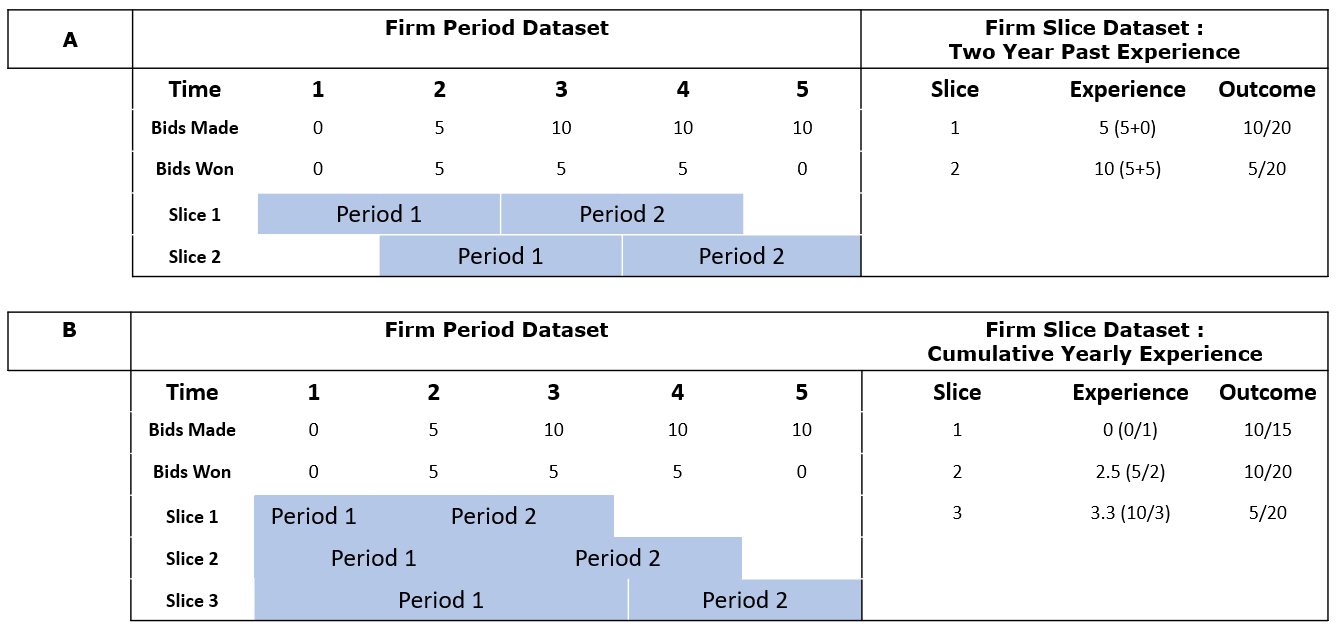
\includegraphics[scale=0.53]{diagram_experiences.png}
  \caption{Example computation of slice-firm dataset, employing two-year fixed periods of past experience (A), and cumulative yearly experience (B).}
  \label{fig:diagram_experience}
  \vskip 0.5mm
  { \footnotesize \underline{Note:} }
\end{figure}

Finally, we add period fixed effects for each period of outcomes being considered to control for changes in the market environment throughout the sample.

%In some specifications we include firm fixed effects based on size. It is possible that smaller firms face higher competition due to less-complex contracts, and so their baseline level of success in the market will be lower.

After the transformation steps, we obtain five slice-firm datasets for the first measure of experience and six slices for the second measure of experience. The following table shows the amount of observations in each slice by the type of experience measure employed. Recall that every observation is a firm-level aggregate of past experience and summary of future outcomes and have the form of the righmost table in Figure \ref{fig:diagram_experience}.


%The OLS regression in equation may have endogeneity problems. This next section discusses the sources of the problem and the identification strategy.


\subsection{Endogeneity and Identification}
Causal interpretation of the regression in Equation \ref{eqn:olsspec} is problematic since unobserved cost variables, specific to each firm, are omitted in the regression (since they are unobservable) and also endogenous. If there are highly efficient firms which due to this advantages are able to bid more aggressively or submit better proposals, they should win more projects, and in turn accumulate more experience. We expect our estimate $\hat{\beta}$ (coefficient on experience) in \ref{eqn:olsspec} to be biased upwards due to correlation (expectedly positive) between omitted cost variables and the amount of past experience.

To identify the causal effect of experience on outcomes, one alternative is to employ external variation to instrument the experience of a firm in an Instrumental Variables (IV) approach. We discuss what would be the optimal way of producing external variation, and, since the data does not allow us to employ this strategy, we propose two second-best alternatives.

Ideally, one could use close wins as the source of exogenous variation in past experience. The argument is that close wins should be less or not at all attributed to unobserved cost factors, or other efficiency advantages, but instead attributable to random differences, for example, the conservativeness of each firms' engineers' estimates. The optimal way to identify close wins would be to single out auctions for which the winning firm had a final weighted score which was marginally superior to the next (or several) of its competitors.  Recall that, for each contract, the  proposals from firms are scored in several criteria, weighted, and finally summed to produce the total score for that firm.

In this approach, our first stage takes the form of Equation \ref{eqn:firststage} . Here $EXP_{it}$ is the total set of contracts won in slice $t-1$ for firm $i$, while $EXPCLOSE_{it}$ is the subset of the contracts won which was won closely as per the definition above, and $\nu_{it}$ is an error term uncorrelated with $EXPCLOSE_{it}$.

\begin{equation}
\label{eqn:firststage}
EXP_{it}= EXPCLOSE_{it}+T_t+\nu_{it}
\end{equation}

The second stage is shown in Equation \ref{eqn:secondstage}.

\begin{equation}
\label{eqn:secondstage}
EXP_{it}= EXPCLOSE_{it}+T_t+\varepsilon_{it}
\end{equation}

Clearly, both measures of experience ($EXP$ and $EXPCLOSE$) are correlated since every extra unit of experience increases the probability of having at least one close win. Moreover, close wins should not be correlated with cost measures, as they are attributed to random factors, such as risk-aversion differences between firms, random approximation differences between engineering teams in each firm, etc. and thus we should also have a valid instrument.

Unfortunately, the previous strategy is unfeasible a with the data we have avalaible. Our data only allows us to see the criteria employed in each contract and the weight of each factor, but not the individual scores for each firm. We attempt two alternative methods detailed in the subsections below

\subsection{Close wins by close bids}
 The first method follows the same theoretical setting as before, but changes how close wins are singled out. Close wins are now operationally identified as the wins meeting copulatively  three conditions: i) the price weight in the awarding decision criteria is 70\% or higher ii) the contract was awarded to the lowest bid and iii) the difference between the lowest bid and the second lowest bid is less than .05\%. We expect that this way of identifying close wins does indeed capture a subset of the random wins, namely, random wins in projects where price is the major awarding criteria.

This definition of close wins leads to approximately 8\% of winning bids being classified as a close one. In the robustness checks, we also consider a different values for these parameters, where we consider close wins where three or more competitors are all within a 1\% difference in their bids.

In the next table we examine whether close wins defined as  above are different from the population in several types of metrics. We can see that in most aspects these bids are not exceedingly different from the rest of the sample, so we expect that there are no underlying project characteristics that could affect competition for these contracts.

\begin{table}[!h]
\caption{Comparison of key statistics between close wins(<0.05\% difference between 1st and runner-up) and regular wins}
\centering
\resizebox{\textwidth}{!}{
\begin{tabular}[t]{ccccc}
\toprule
Variable & Mean (Not close win) & Mean (Close win) & Sd (Not close win) & Sd (Close win)\\
\midrule
Bid & 6.3e+08 & 3.32e+10 & 1.06e+10 & 8.11e+12\\
Bid\_Winning & 3.18e+08 & 2.37e+08 & 3.56e+09 & 2.62e+09\\
Difference between 1st bid and 2nd (\%) & 0.14 & 0.0186 & 0.115 & 0.0147\\
Number of Bidders & 3.86 & 4.08 & 2.12 & 2.23\\
Year & 2020 & 2020 & 2.92 & 2.89\\
Offers made by Firm & 4.4 & 6.17 & 7.34 & 11.2\\
Win prob. by Firm & 0.191 & 0.171 & 0.3 & 0.274\\
Offers won by Firm & 0.972 & 1.37 & 2.1 & 3.23\\
\bottomrule
\end{tabular}
}
\end{table}

\subsection{Close wins as close rank}
There coul two main objections to the previous identification strategy:
\begin{itemize}
  \item The price is not the only awarding factor. Thus, it is possible that even in a contract where price is a major component, the cost advantages of a firm manifest in terms of other awarding factor, like quality. That is, the firm offers similarly priced goods but at a much superior quality.
  \item The closeness between the first and the second bid does not take into account the full pool of participants.
\end{itemize}

We propose a new alternative to identify close wins which does not rely in prices or any other aspect of the bid itself. Instead, we label for any winning given firm a close win if all the firms involved in the auction were close in ranking. The argument here is that, given a well constructed ranking, winning a contract against closely placed opponents is attributable to random factors.

Obviously, the main issue is how to construct a good ranking measure. We proceed by  modeling each auction as a multi-player game event (in the non-economic sense of the term) in which firms gain points by winning the project and lose points by not winning it. We award and substract points based on a modified ELO algorithm suited for multi-player games.

Each firm has its ranking initialized at a pre-specified level (1,500 in the initial version). Then, it is awarded 24 points for winning againsta a similar oponnent and substracted 8 by losing. The implementation of the algorithm recommends that points awarded and substracted sum to zero, so we fix awarded points and choose substracted points such that on average (given the number of players in an auction) this condition holds. Against non-similar opponents, the algorithm makes a correction based on the ranking of the players and the outcome of the game. The details of the algorithm are given in the Appendix.

Proceeding from the oldest to the most recent auction, we update the initial rankings for each firm and obtain for each firm its ranking at any point in time. Next, we label a win as a "close win" when the highest rank among the bidders for the auction was not more than 3\% higher than the lowest rank among the same set of bidders. This yields around 7,322 closely won contracts (16\% of the contracts in the analysis sample) which corresponds to 21,763 observations (16\% of the observations in the analysis sample). In Table \ref{tab:closewins_alt2_desc} we present summary statistics for close wins identified via close wins.

\input{C:/repos/learn-doing/thesis/tables/table_closewins_alt2_desc.txt}

In the analysis, for our first measure of experience we drop the first slice of data outcomes (as defined above) to allow for a period of rank adjustment. This is necessary since the algorithm does not work well when the average rank in the population is not clearly defined. The way ranks evolve as we progress in the time of the data can be seen in Figure \label{fig:rankings_times}. Note that ranks appear concentrated at the end of the first year of data, while much more dispersed at the end.

\begin{figure}
  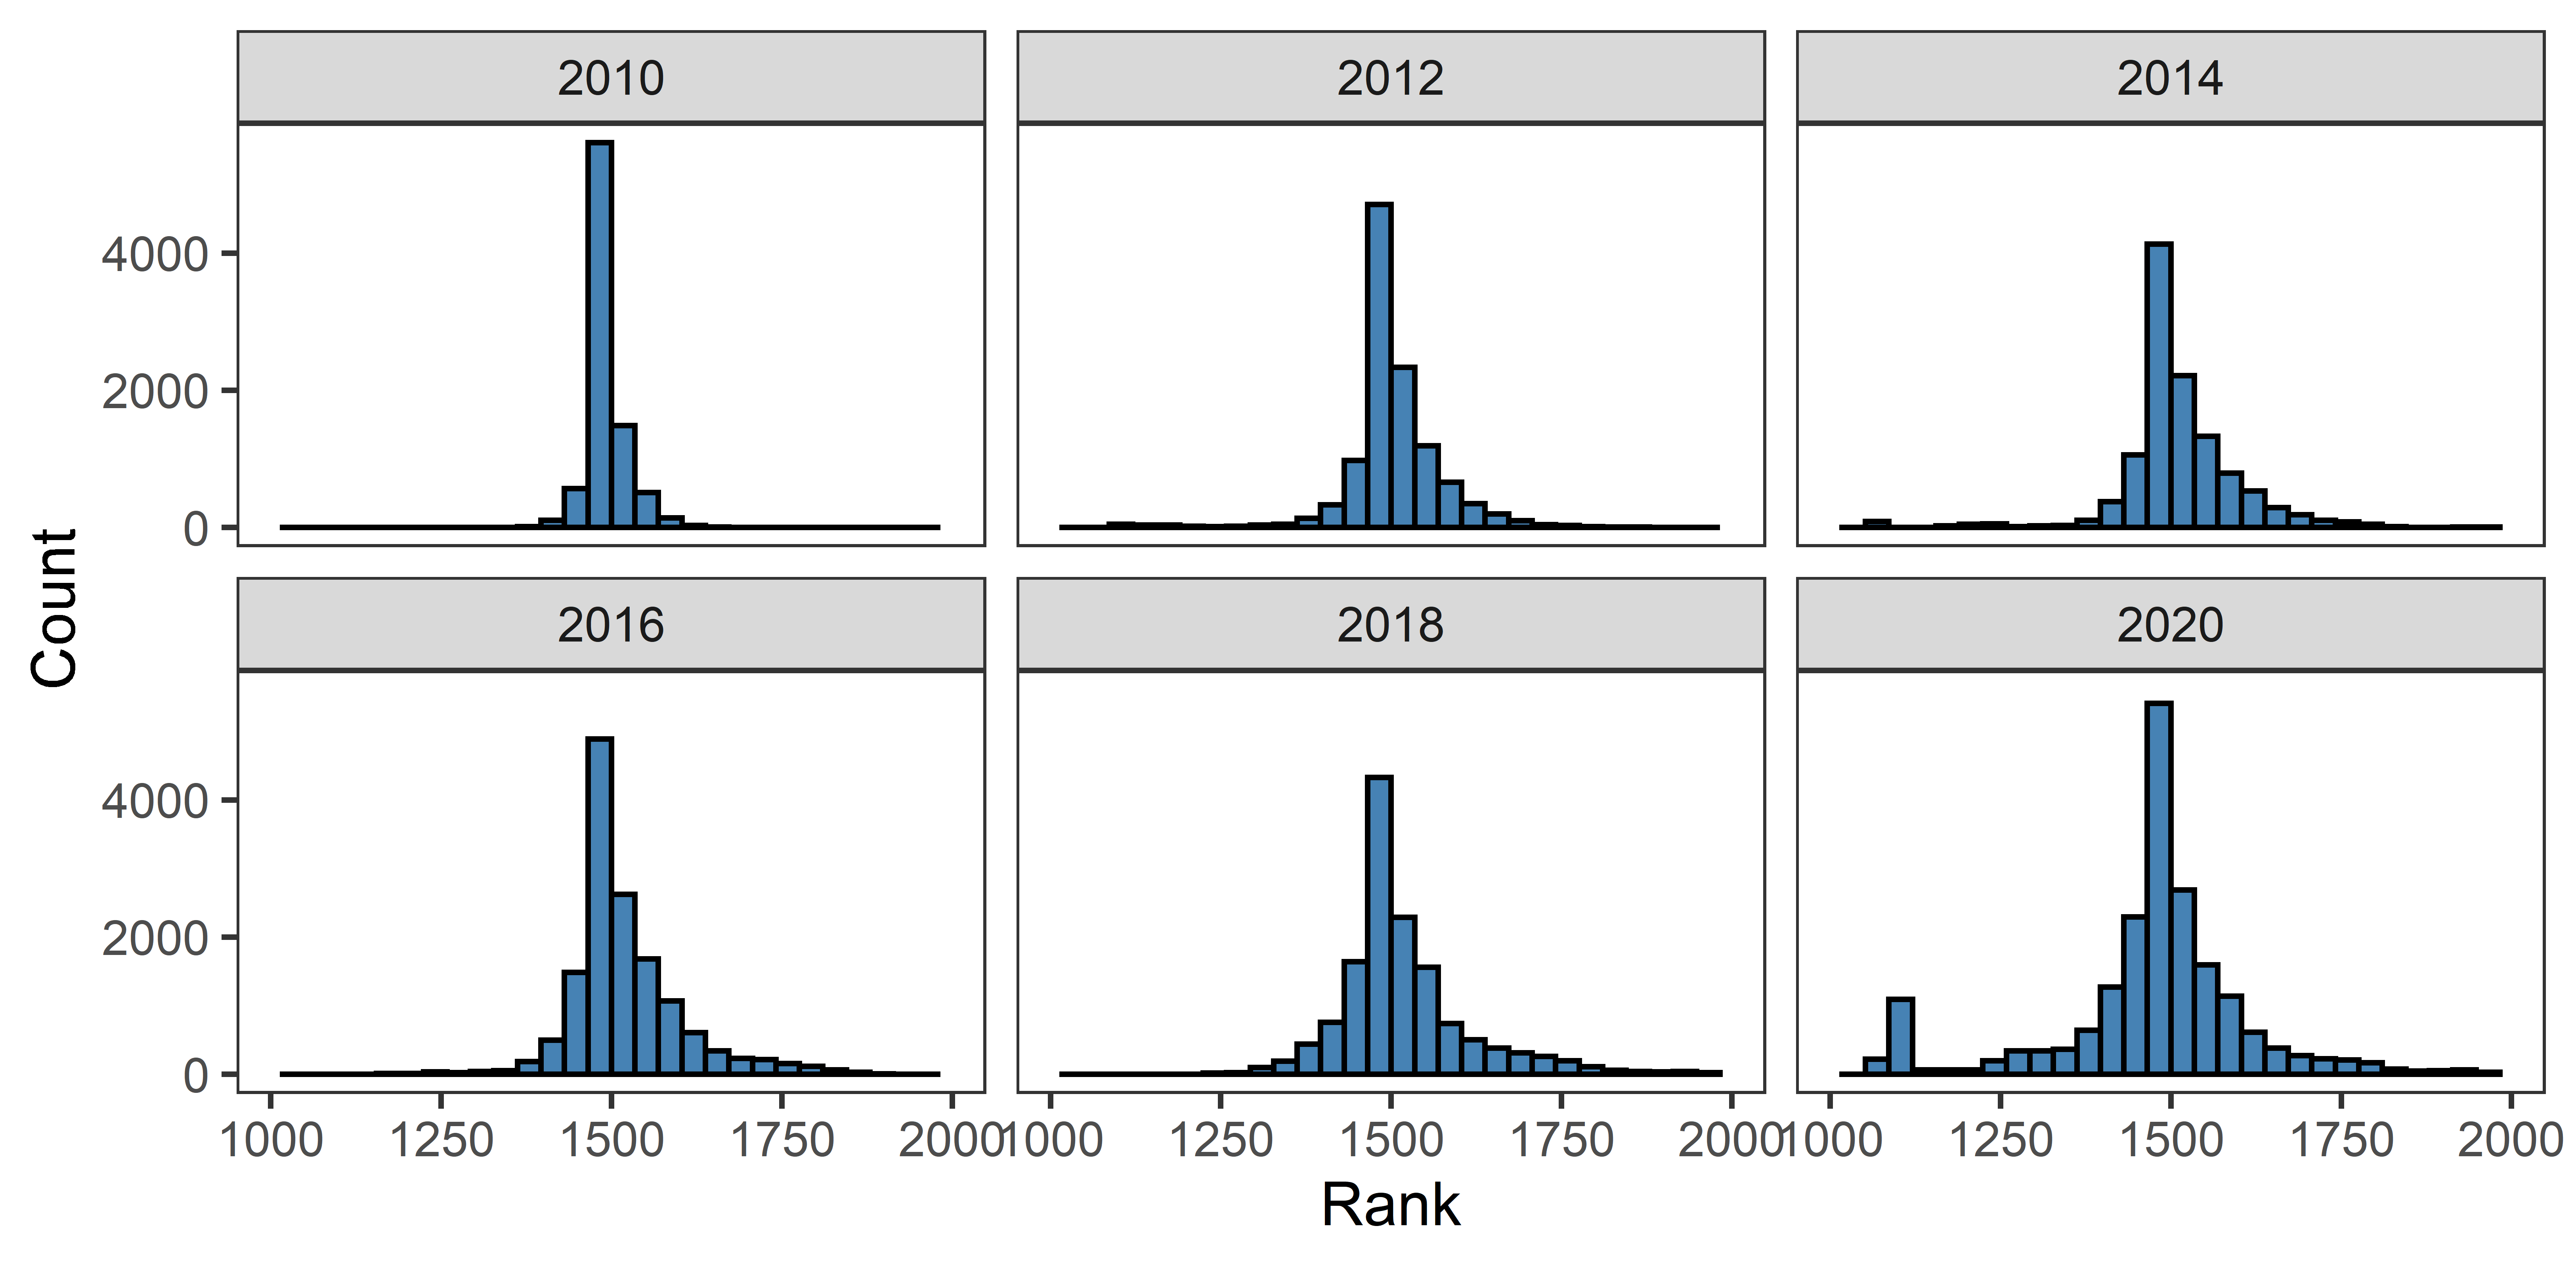
\includegraphics[scale=0.95]{rankings_times}
  \caption{Evolution of ranks by selected years}
  \label{fig:rankings_times}
  \vskip 0.5mm
  { \footnotesize \underline{Note:} \par}
\end{figure}

In the robustness checks we analyze both i) different values for the won/lost points after an auction and ii) the threshold in ranking for a close win.
%Bidding behavior
%An alternative way to measure changes in bidding behavior caused by efficiency gains through experience is to examine directly changes in bidding behavior among more experienced firms with respect to less experienced ones. As was discussed before, experience induces changes in the underlying production function, or changes along the production function, that make the firm more efficient at producing certain types of goods. In a competitive market, firms should pass through at least a fraction of this improvement in costs to the bids they submit in the auctions. Thus, we should be able to identify this change directly through the bids that more experienced firms submit for projects.
%The approach is different than the one from the previous section because we can directly link the past experience of a firm to each bid it submits in every auction that it participates in. Thus, our unit of observation is a bid submitted by a firm for a contract of a public construction contract. Our second specification has then the following form:where is the standardized bid submitted by the firm and is a measure of past experience. In further specifications we include a broader set of controls. First, we add fixed effects by auction. Second, we add firm fixed effects. Finally, we control by the geographic region where the auction is being held.
%The outcome variable is the standardized bid submitted by firm to the auction, i.e. the original bid amount divided by the engineering estimate of the project. This approach allows us to make comparisons along project of different sizes. It is also useful because it should be expected that our dependent variables have effects per unit of contract amount (Bajari, 2010). The standardization also controls for some sources of heterogeneity.
%The dependent variable is the total number of contracts that the firm has won up until the moment that the firm submits its bid. Since for the first periods in the data we do not have information on past experience, we exclude the first two years from our observations of outcomes and only employ them to compute experiences for firms from year three and onward. In the robustness section, we explore several alternative ways to measure experience and subset the set of firms.
%In the same way as before, we expect that there will an endogeneity between cost measures and bidding behavior. We should expect that firms which have a baseline efficiency higher than other firms will be able to submit lower bids and gain more experience, so we could pick up effects of reverse causation in our coefficient for experience.  We thus employ a similar Instrumental Variables approach as before, instrumenting total past contract wins with close contract wins.

\section{Main Results}

First we explore graphically the relationship between our first measure of experience and outcomes. Figure \ref{fig:plotresults_both} , Panel A, shows the relationship between past experience and outcomes (i.e. winning share). While we can see an increase in the average share of contracts won with more past experience, there is considerable heteregeneity, as it can be seen in the wide error bars (which show interquartile range). Panel B contains only two types of firms: firms that either bid but not won contracts in period $(t-1)$ or firms which won one or more close contracts in period $t$, and thus is akin to results of a reduced form regression.

\begin{figure}
  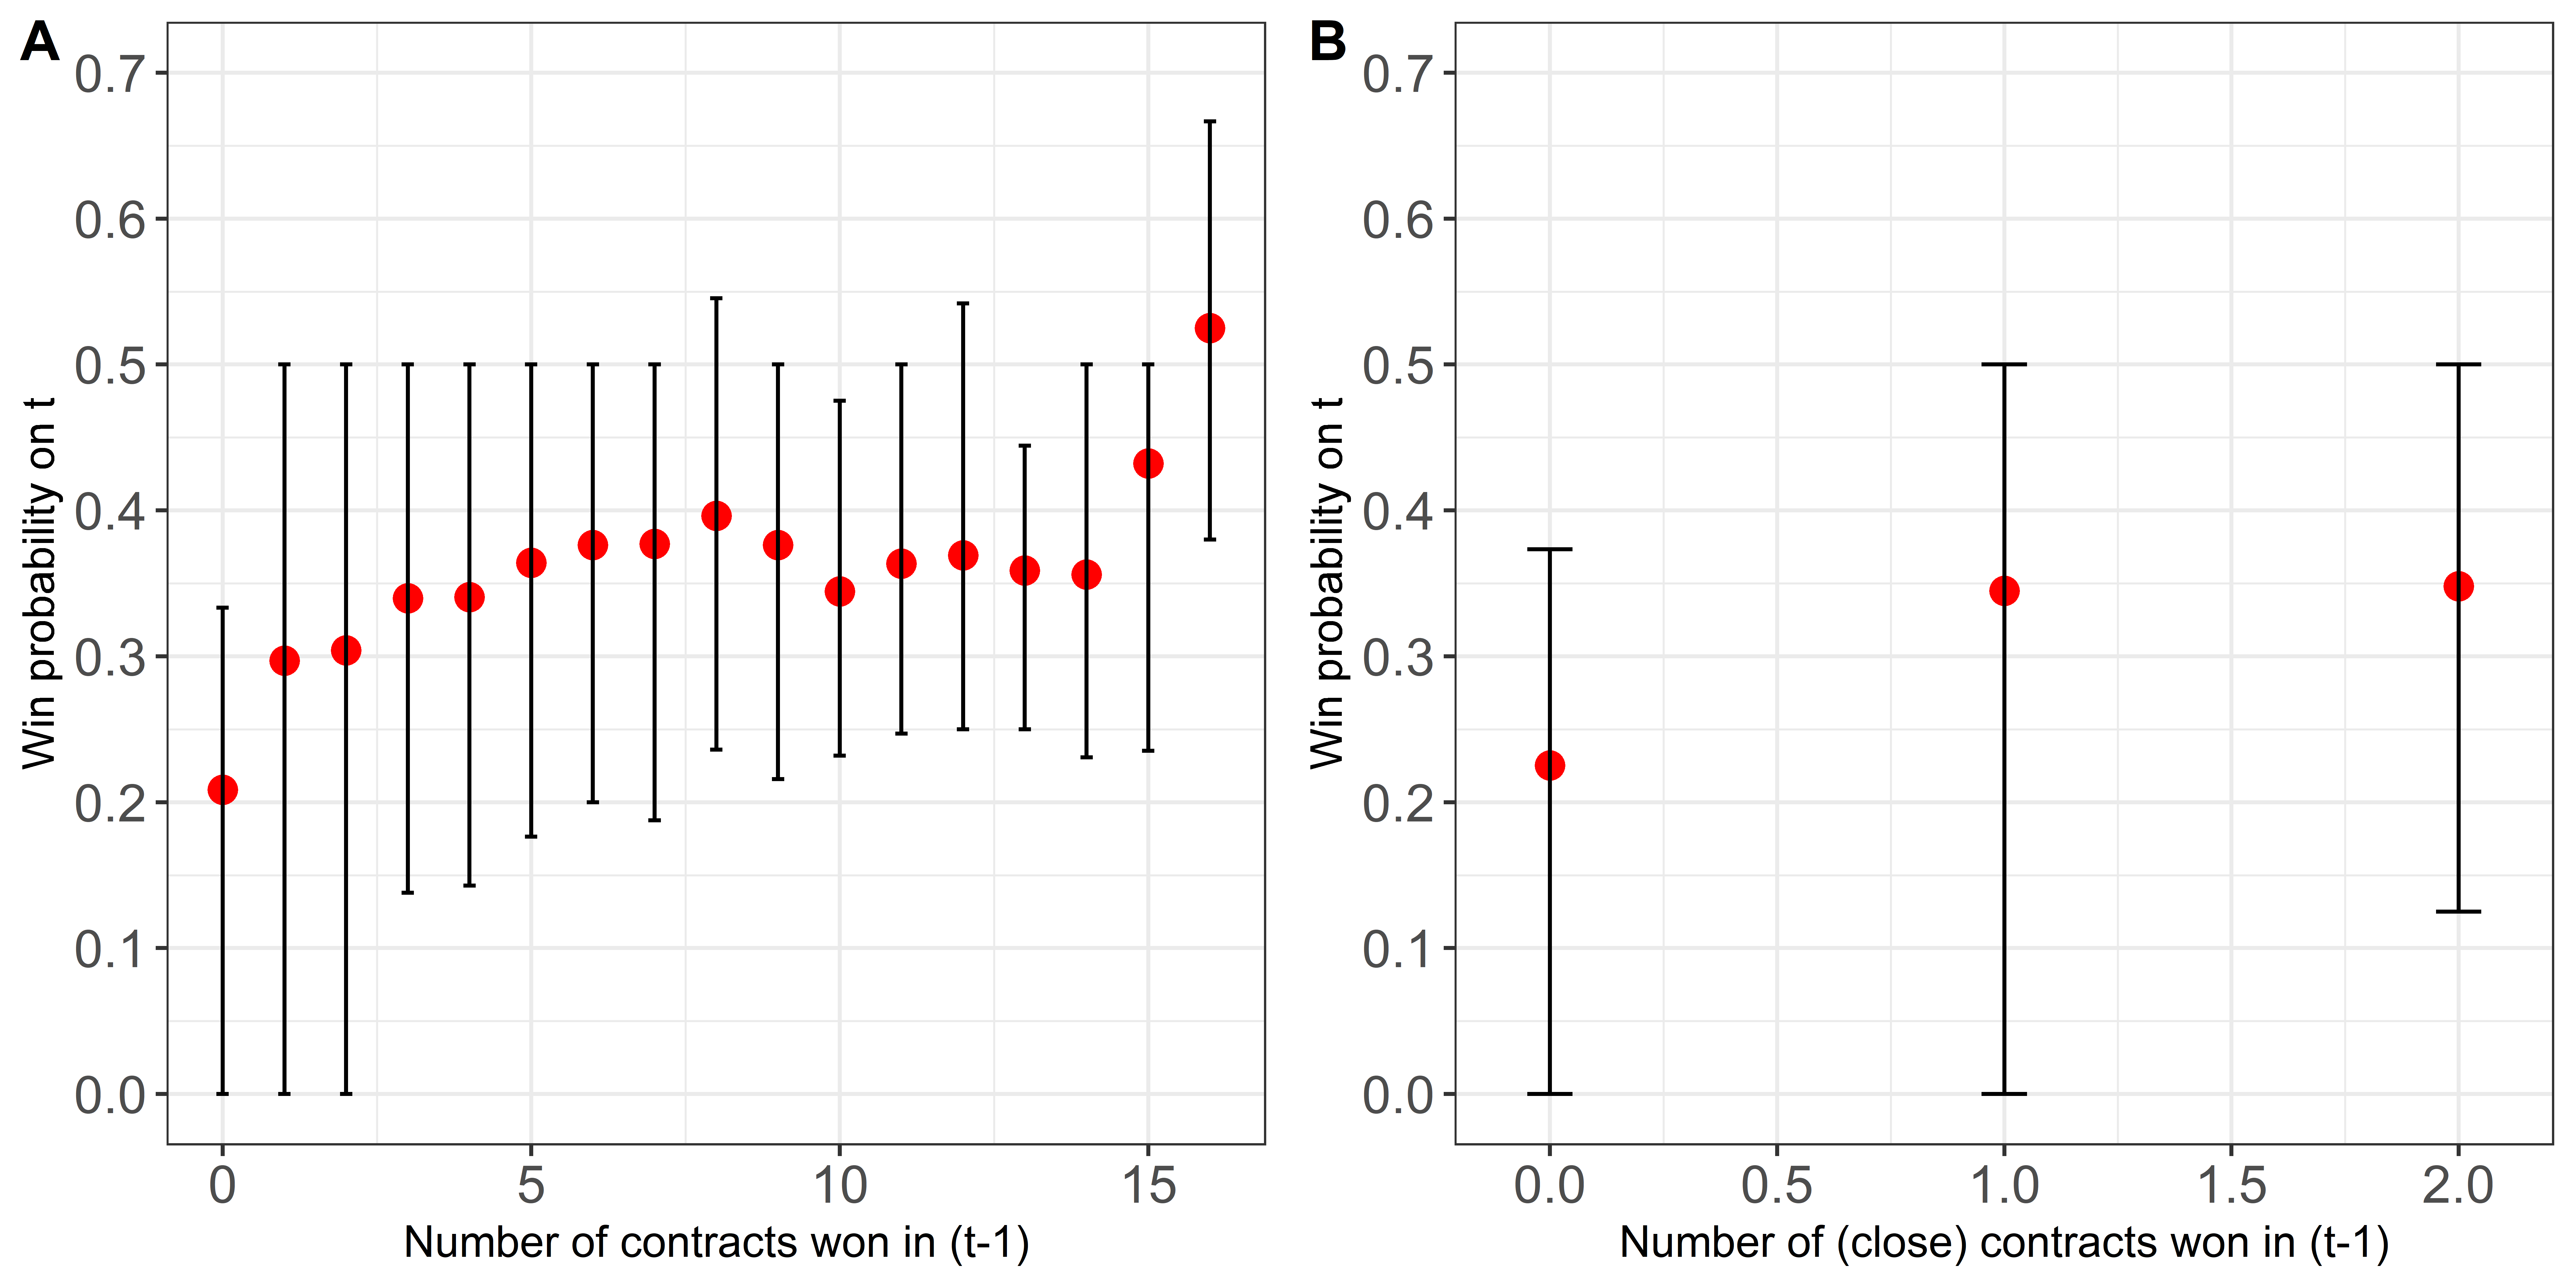
\includegraphics[scale=0.65]{plotwins_both.png}
  \caption{Relationship between contracts won on $t-1$ and mean winning probability across contractors in $t$.}
  \label{fig:plotresults_both}
  \vskip 0.5mm
  { \footnotesize \underline{Note:} The plots show the mean across firms of the number of contracts won out of the number of contracts bid for in period $t$ (in the $y$-axis), against experience accrued in period $(t-1)$ in the $x$-axis. $t$ and $t-1$ correspond to two periods of two years each. Since the data contains ten years, the observations correspond to outcomes computed for eight outcome periods.  Only $x$ for which the number of observations is greater than ten are shown. Error bars correspond to the interquartile range. Panel A: all sample observations are considered. Panel B:  shows results for a subsample where the only contractors considered are those who either i) won closely one or more close contracts  on period 1 or ii) did bid but not win a contract in period 1\par}
\end{figure}

Table \ref{tab:table_exp_1} shows the results for OLS and IV regressions for our first experience measure (i.e. rolling two year periods) while Table \ref{tab:tableExp2} shows the results for our second measure of experience (i.e. annualized experience).

In both tables, OLS results are in the first to third panels. The first panel shows that the OLS coefficient on the effect of having any level experience against not having experience (binary) is around 0.10, for both ways of computing experience (and ). Our specification with linear returns on experience shows that experience renders a 0.02 and 0.05 increase in winning share per extra contract developed (for experience measures 1 and 2 respectively). All the estimates for the experience-related coefficients are significant at $p=0.01$ with robust standard errors.

The IV results (fourth to sixth panels in each table) show that  the linear and quadratic estimates of the coefficients on experience generally stay within $\pm$ 0.03 of their OLS counterparts. There is however an increase in the binary measure of experience coefficient, for both measures of experience, since for the first measure of experience \textbf{this rises from and for the second measure this rises from} . This is different than we expected, as our initial concern was that omitted cost variables would bias estimates upwards.

A concerning result is the low $R^2$, which shows that altough the effect of experience on the mean outcome is significant, there is much variability among firms' outcomes which is not explained by experience.

\input{C:/repos/learn-doing/thesis/tables/table_ols_exp1.txt}

\input{C:/repos/learn-doing/thesis/tables/table_ols_exp2.txt}

There does not seems to be conclusive evidence regarding different results when employing quadratic rather than linear functional forms for experience. For example, Figure \ref{fig:pred_average} shows the mean confidence intervals, employing as period fixed effects the last period in the sample. It can be seen that the fitted total predicted value does not seen to vary greatly from the linear to the quadratic specification.

\begin{figure}[H]
        \centering
        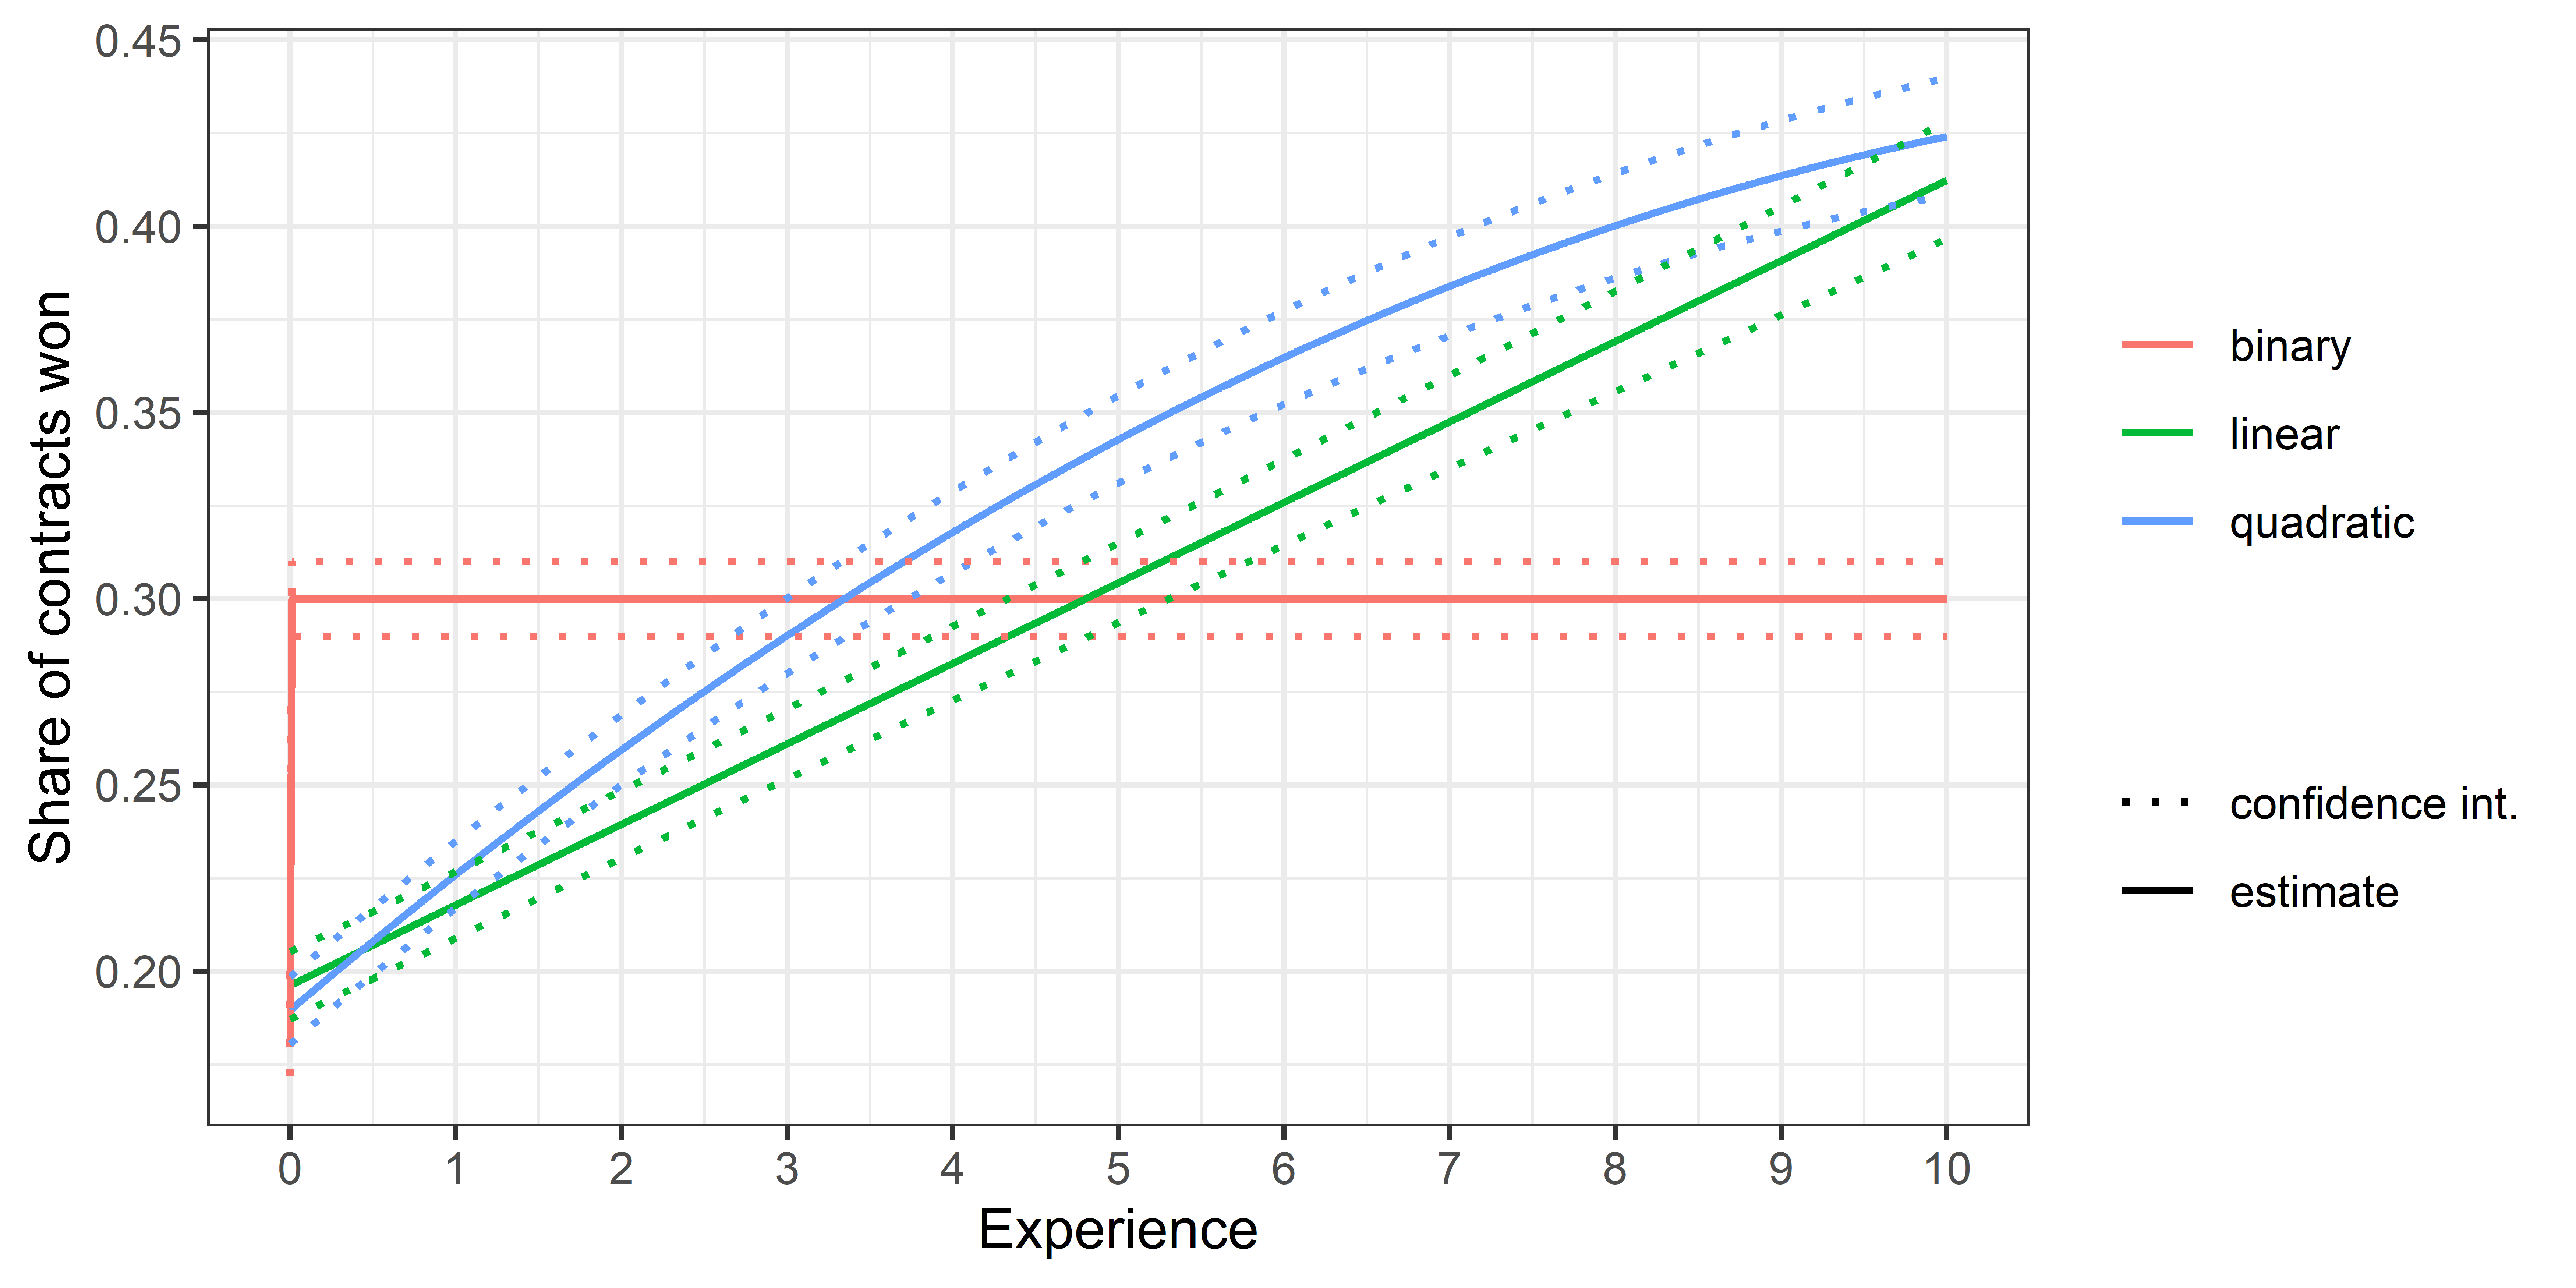
\includegraphics[scale=0.8]{fit_sample.png}
        \caption{ \small Predicted values for the mean of the outcome variable (share of contracts won), by total experience accrued in the previous period. We employ fixed effects as in the last period of the dataset.}
        \label{fig:pred_average}
    \end{figure}




\section{Experience and Type of Project}
Given our previous results a natural concern is if whether all projects exhibits the same returns to experience or if experience is more important in certain types of works. In this section we replicate the previous analysis by disaggregating by type of project. In order to do this, we classify certain projects according to their description, then run similar regressions as in the last section, and present the results.

First we describe briefly how we construct categories for the prrojects and which ones are avalaible for the analysis. Our original dataset includes a name variable which describes the type of project with some extent. We extracted this name variable and looked for i) common single words (unigrams) and ii) common pairs of words (bigrams). We select the most common unigrams and bigrams and map similar words and bigrams to project categories. The full categorization mapping can be found in the Appendix.

We end up with contract classified under categories. Importantly, if a contract includes unigrams or bigrams in its name belonging to more than one category, it is included in the analysis of both categories. The number of contracts, average amount, average number of bidders for each category is shown in Table \ref{}. We can see that the biggest categories of projects are school-related, vecinal works, parks and pavements (including sidewalks). The Appendix contains more details on the types of projects included in each category.

%\input{C:/repos/learn-doing/thesis/tables/table_types_project_stats.txt}

Next we run similar regressions as in the previous section for each project type, considering as our dataset only the contracts in that project category . We employ the same specification of with a linear functional form on experience and period fixed effects, and our first measure of experience. The results are presente in Figure \ref{fig:typeestimates}he Appendix includes more detailed tables with full regression results for each sproject type. A few results stand out. First, we get the biggest coefficients on experience on graveyard projects, footbridges and housing. The first two should be almost exclusively procured by government units. Housing was also one of our hypothsized types of projects which should have high coefficients. At the bottom of the distribution, interestingly, we find daycares, sports courts, hospitals, and schools. The results could be explained because these projects are mostly composed of normal construction works which also have private close substitutes.

The results on hospitals should be surprising, as they are usually very big projects with a lot of specific knwoledge required.

%\input{C:/repos/learn-doing/thesis/tables/table_types_project_ols.txt}

\begin{figure}
  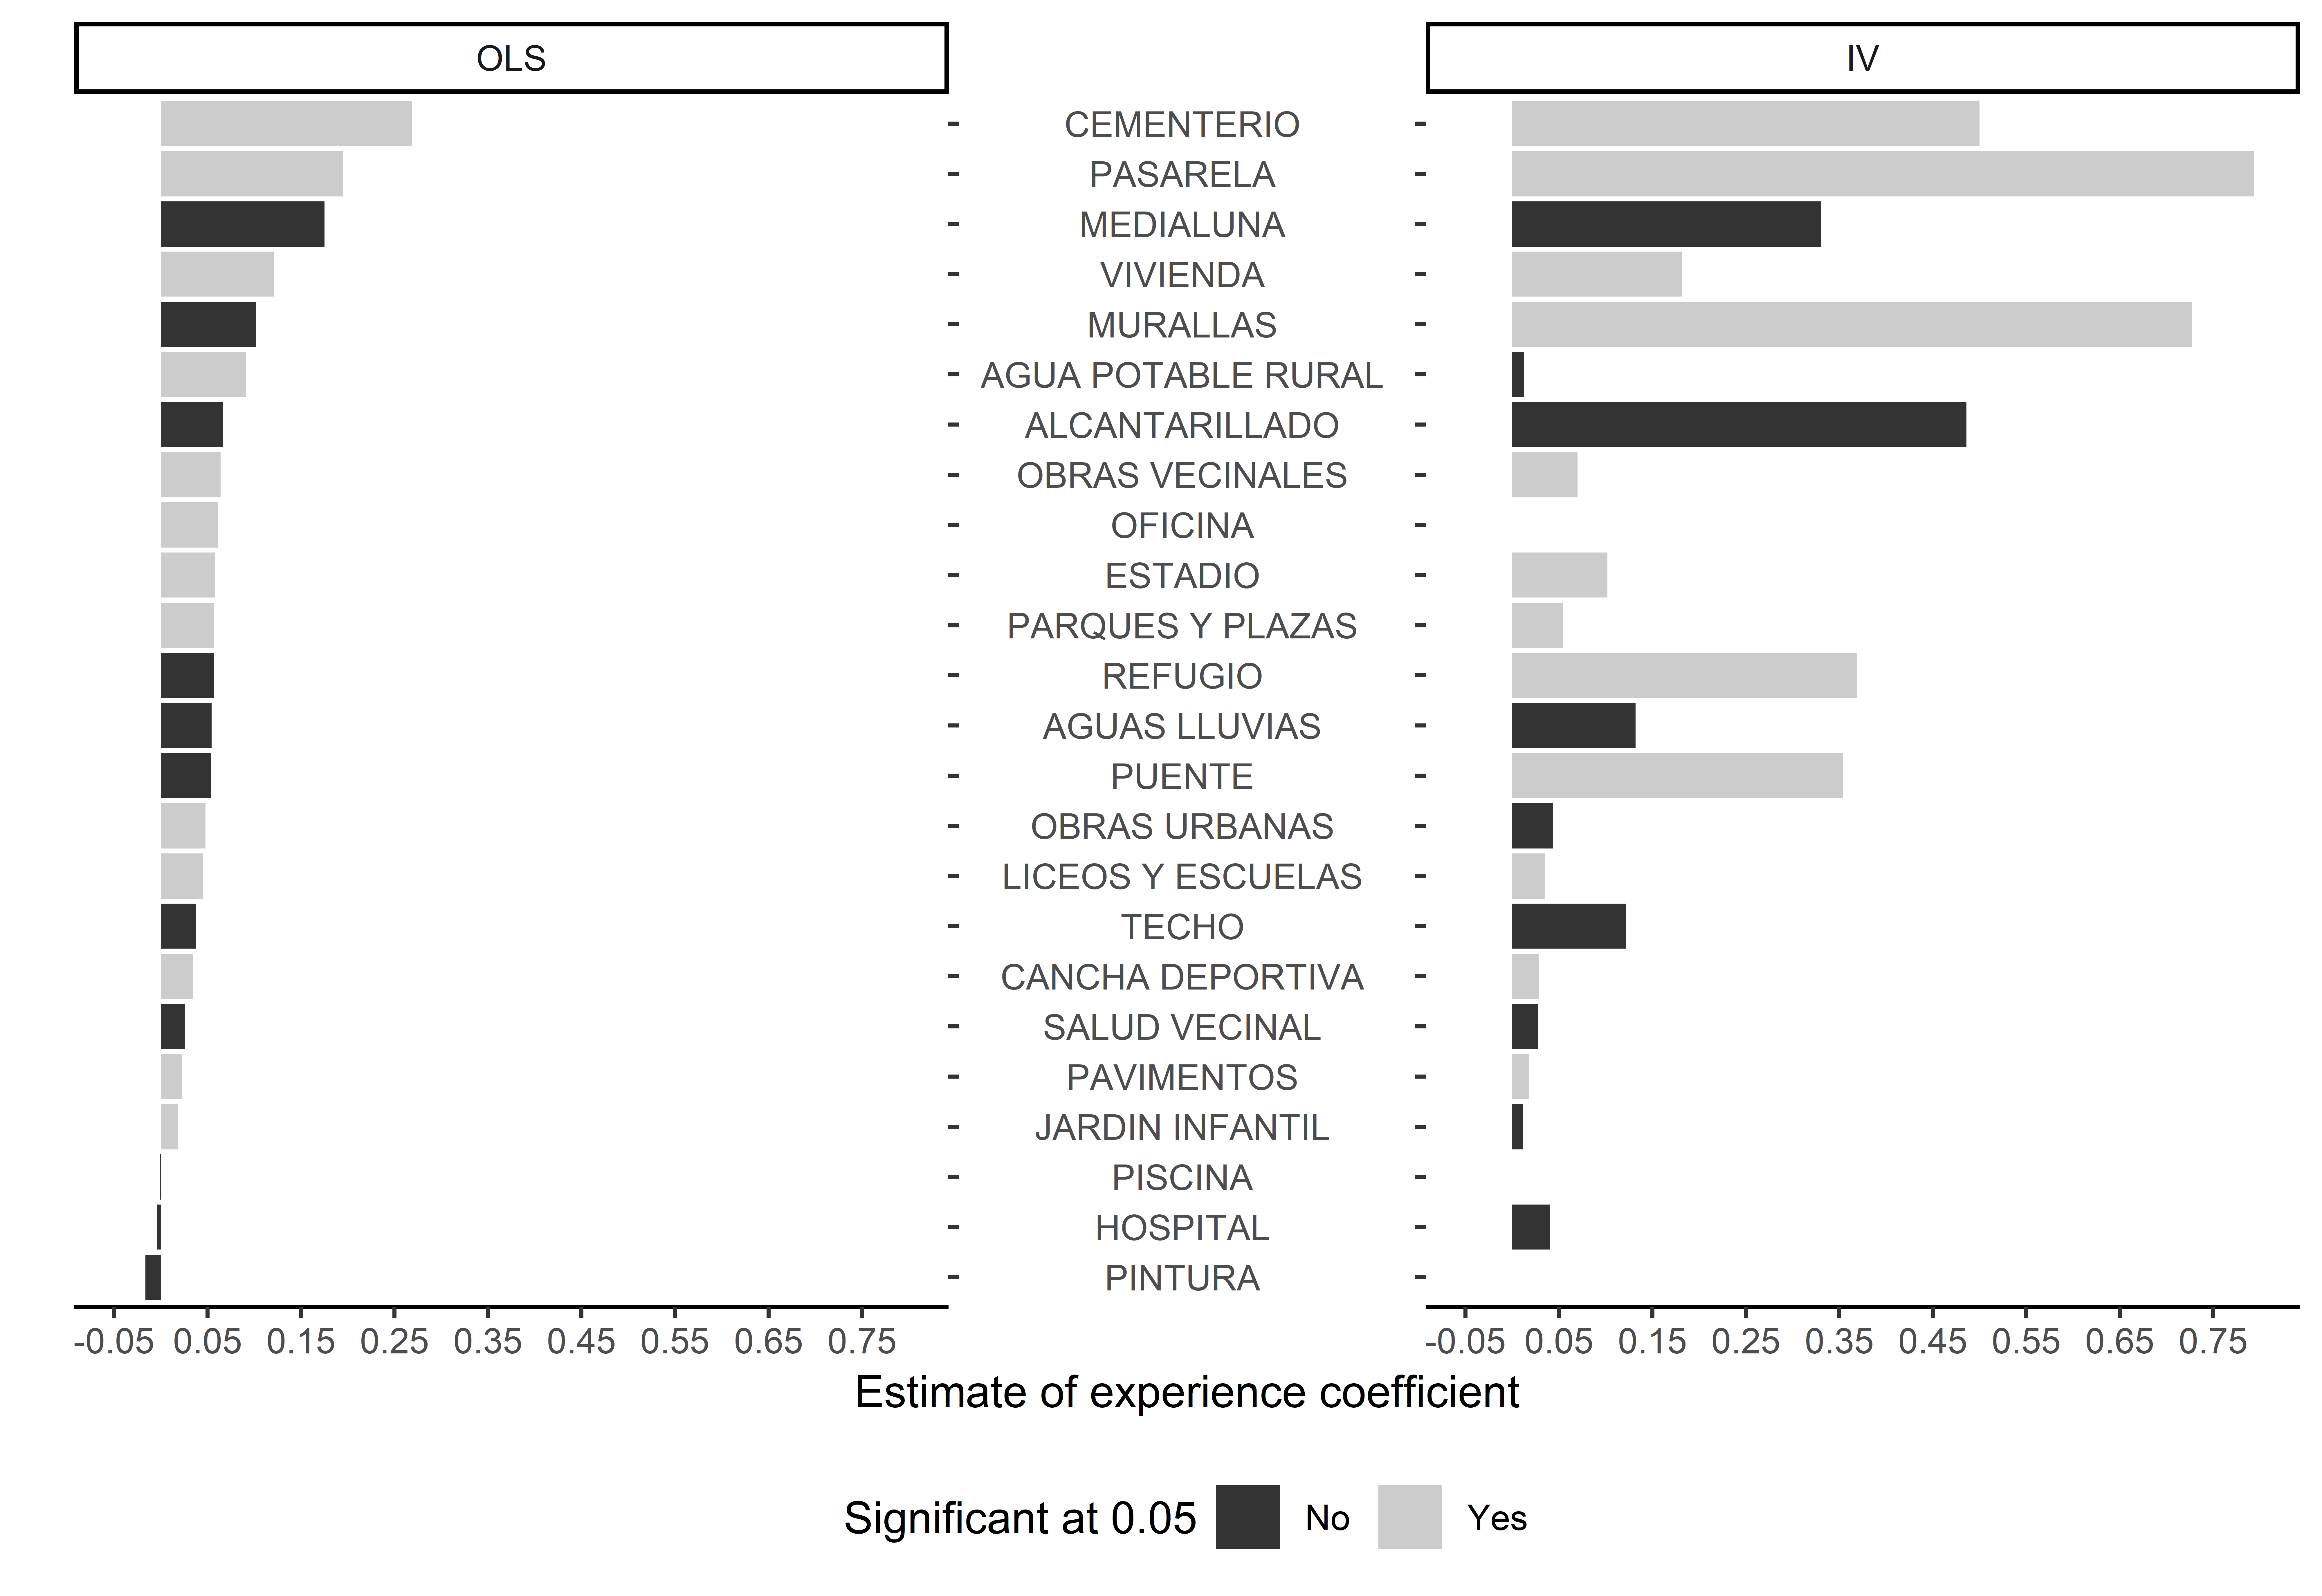
\includegraphics[scale=0.75]{plotTypes.png}
  \caption{Experience coefficient by type of project.}
  \label{fig:typeestimates}
\end{figure}

\section{Experience and Firm Size}
%In the literature about industrial organization and productivity, it has been studied the relation between firm size, innovation, and productivity. These investigations have concluded that smaller firms are more productive than bigger firms, however they are also more risky.
An important variable in the investigation of the effect of experience should be firm size. First, it is possible that there are different levels of cost efficiency between small and big firms. As arguably bigger firms should have more experience on average, this could skew our estimates. A second concern is that we might expect experience to matter more for smaller firms, if there is a decreasing or "maximum" level effect of experience on future outcomes.

In this section we attempt to develop specific estimates of the effect of experience for different levels of firm size. Developing intra-category estimates serves as both as an identification strategy and as  robustness check of our previous findings.

 We follow the following approach. First we select a subsample from our original dataset which we can classify acoording to annual sales.  We obtain intra-category estimates of the effect of experience and interpret them. Finally, we discuss the results and some of the empirical challenges of controlling for size.

In order to study and control for firm size we employ a publicily avalaible classification of firms according to their annual sales, maintained by the chilenan Tax Bureau Office (\textit{Servicio de Impuestos Internos}). Firms are categorized in 13 categories. Category number one  corresponds to 'tax data not enough to classify', but from categories two up to thirteen, each category is defined by an increasing level of minimum yearly sales.

This data is avalaible only for firms not being fully assimilable to final taxpayers. After merging our with our initial sample, we are left with around 30\% of our original firm sample. Table \ref{tab:salescategories} shows how many firms do we have in our sample for each category, average annual sales for these firms, and statutory annual sales thresholds for each category. Note that we have much more firms at intermediate categories than extreme ones. In our estimation we group firms from contiguous groups together to increase power.

% Table generated by script
\input{C:/repos/learn-doing/thesis/tables/table_tax_categories_data.txt}

We estimate the effect of linear experience with our first measure for each group of categories of firms by OLS and IV. Specifications consider our first measure of experience with a binary presence of experience and with period fixed effects. The results are presented graphically in \ref{fig:sizeestimates} (the coefficient for category two is omitted because it was much bigger than the rest and distorted the visualiztion). Full results are avalaible at the Appendix.

We only obtain significant effects at intermediate sales categories' levels. However, everytime a coefficient is significant it is also positive. The results are not supreising given i) the reduced sample we are employing ii) the expected reduced importance of experience for very big firms.

Controlling for firm size is challenging mainly because of statistical reasons. First, firm size distribution in the sample is not uniform as there are less very small and very big firms. Second, the within-size distribution of experience within extreme categories has very few observations with more than five contracts of experience. Third, this sample is already smaller due to filtering single-person companies. Both factors make it hard to obtain per-category estimates with enough statistical power experience.

\newpage
\input{C:/repos/learn-doing/thesis/tables/table_firm_sizes_intercepts.txt}


%\begin{figure}
%  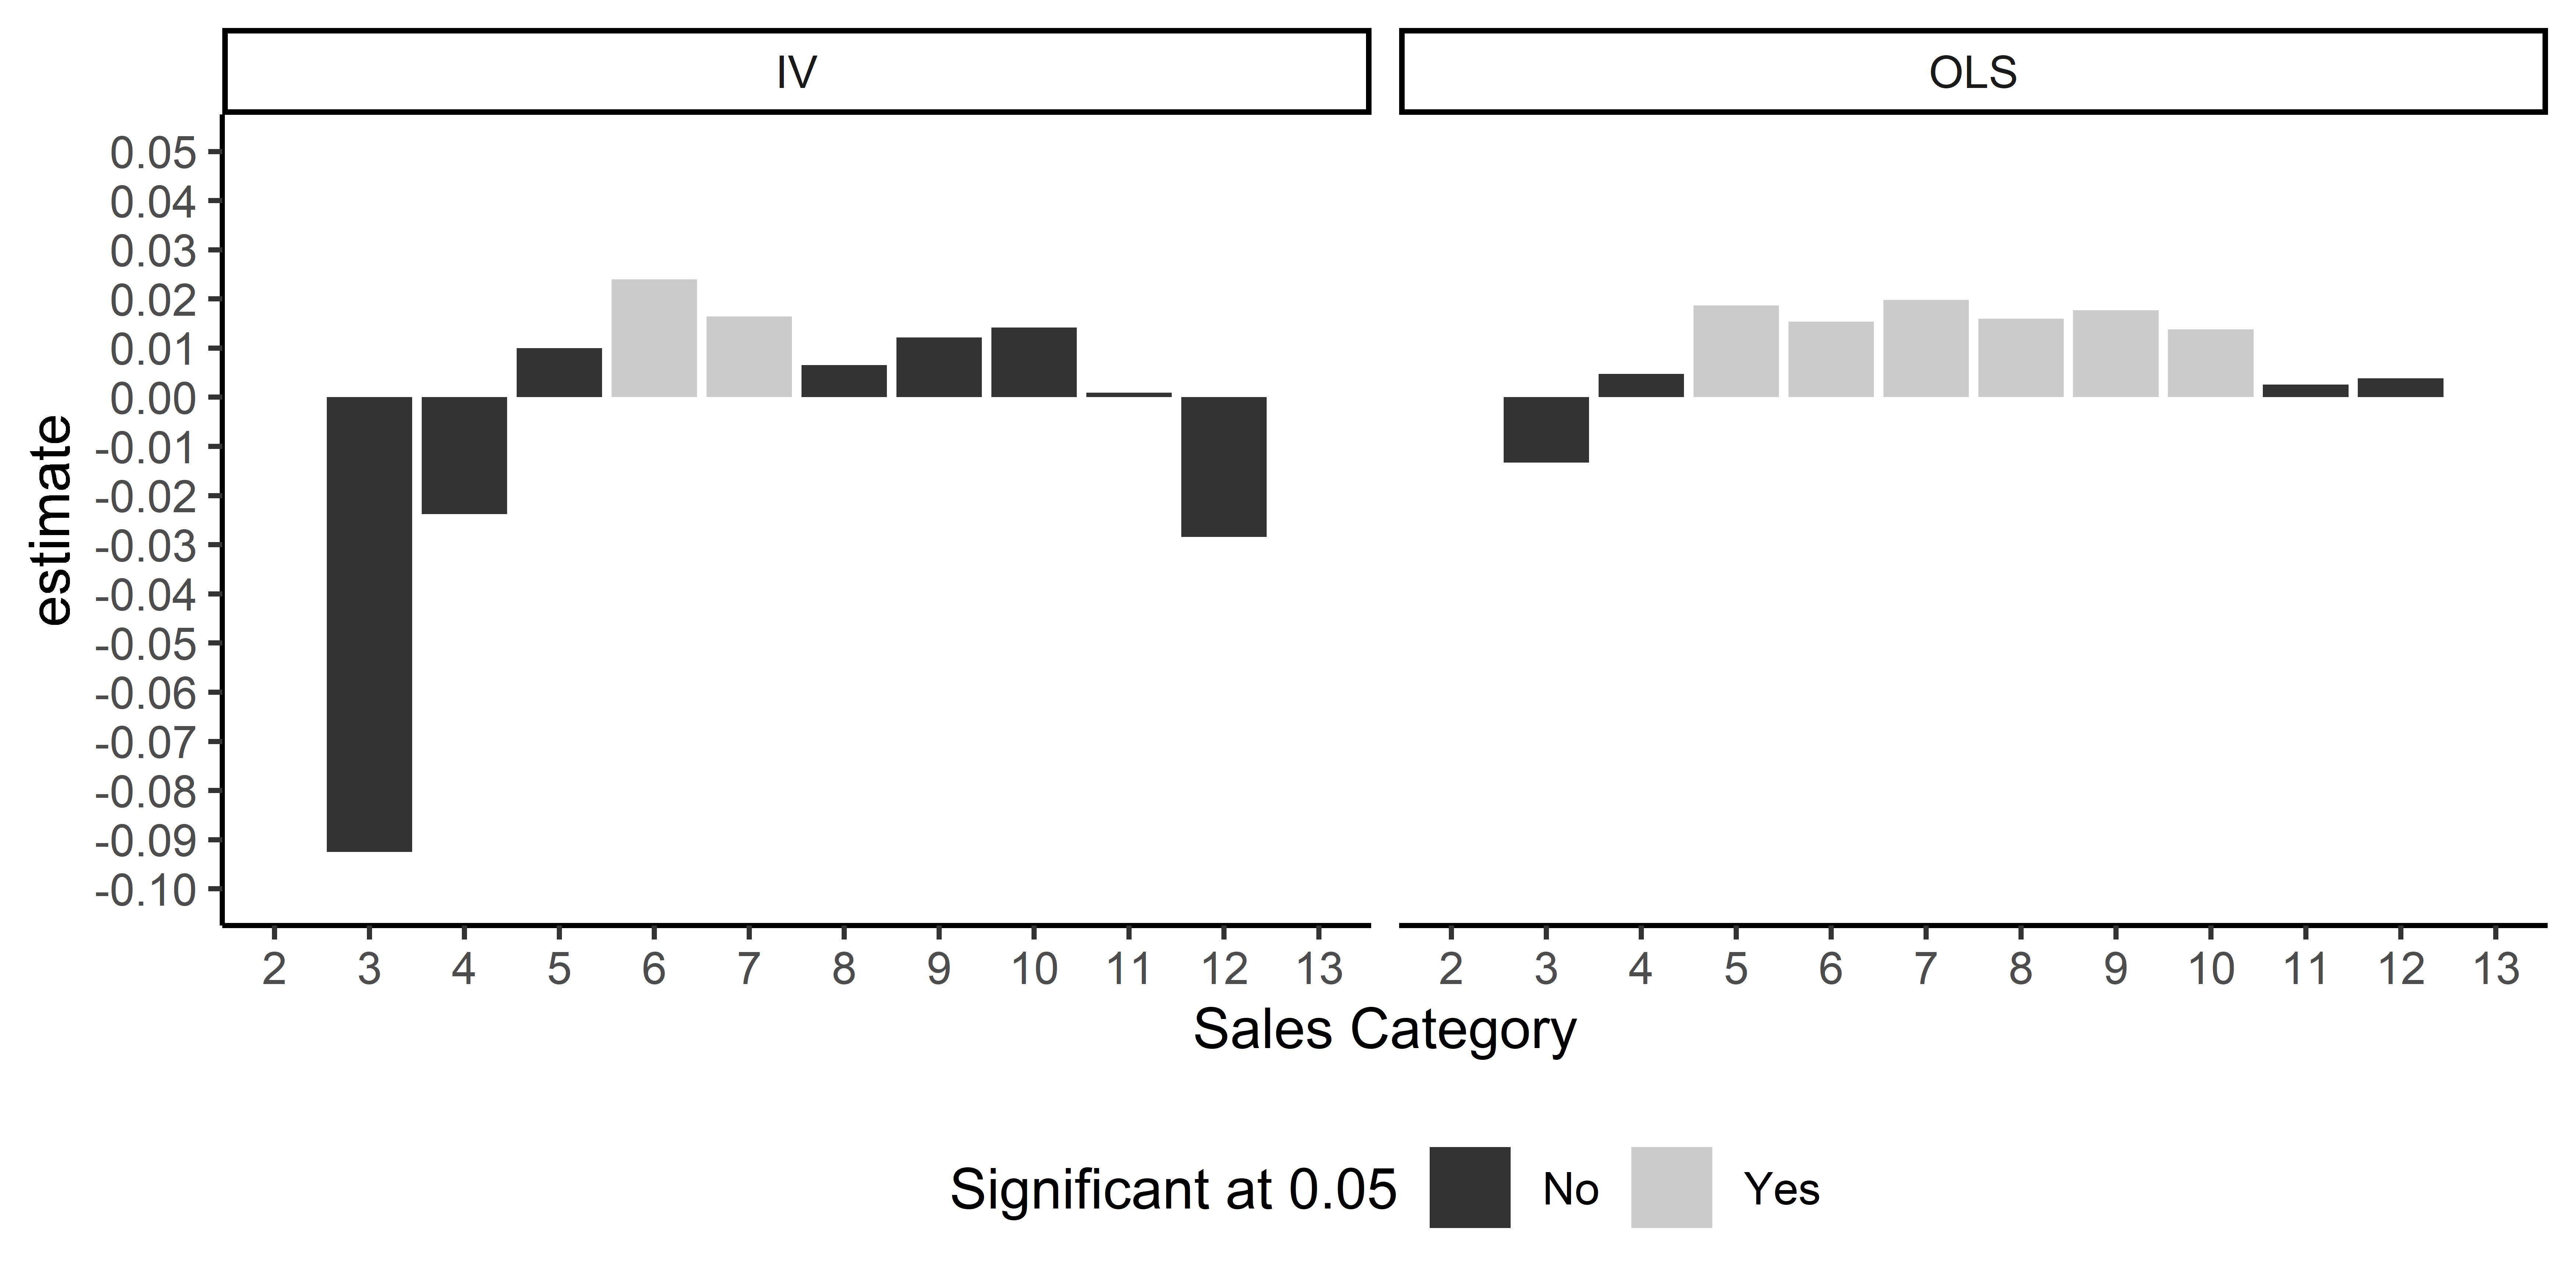
\includegraphics[scale=0.85]{plotsize.png}
%  \caption{Experience coefficient by tax sales category}
%  \label{fig:sizeestimates}
%\end{figure}


%\resizebox{\textwidth}{!}{%
%\input{C:/repos/learn-doing/thesis/tables/table_sizes_explinear1.txt}
%}%
\section{Robustness checks}
Several of our choices in the previous section admit several arbitrary choices. In this section we consider several extensions in parameters which could influence the results obtained before. We consider robustness checks in the following areas:

\subsection{Periods of outcomes}
In the previous section, we measured outcomes occuring in two year periods. We now consider outcomes occuring in one and three year periods as well. Note that in this part we only vary the length of the period where outcomes are computed and we maintain the procedure to compute experience as before. Table shows outcomes computed for periods of 1, 2(the original specifications) and 3 years. The first three columns employ the experience measured in the two-period previous to the outcome period while the 3-6 compute experience as annualized cumulative experience as discussed in the previous section.

\begin{table}[!htbp] \centering
\caption{Regression for OLS and IV specifications}
\label{}
\resizebox{\textwidth}{!}{%
\begin{tabular}{@{\extracolsep{5pt}}lcccccc}
\\[-1.8ex]\hline
\hline \\[-1.8ex]
& \multicolumn{6}{c}{Contracts Won/Contracts Bid in Outcome Period} \\
\cline{2-7}
\\[-1.8ex] & \multicolumn{6}{c}{Outcome period of length (years):} \\
& 1 & 2 (Original) & 3 & 1 & 2 (Original) & 3 \\
\hline \\[-1.8ex]
Experience & 0.022$^{***}$ & 0.020$^{***}$ & 0.023$^{***}$ &  &  &  \\
& (0.001) & (0.001) & (0.001) &  &  &  \\
& & & & & & \\
Annualized Cumulative Experience &  &  &  & 0.060$^{***}$ & 0.058$^{***}$ & 0.061$^{***}$ \\
&  &  &  & (0.002) & (0.002) & (0.002) \\
& & & & & & \\
Constant & 0.270$^{***}$ & 0.309$^{***}$ & 0.256$^{***}$ & 0.281$^{***}$ & 0.257$^{***}$ & 0.260$^{***}$ \\
& (0.005) & (0.005) & (0.004) & (0.005) & (0.007) & (0.004) \\
& & & & & & \\
\hline \\[-1.8ex]
Observations & 38,739 & 29,415 & 43,453 & 37,623 & 28,234 & 42,358 \\
R$^{2}$ & 0.028 & 0.031 & 0.025 & 0.026 & 0.028 & 0.023 \\
Residual Std. Error & 0.316 (df = 38730) & 0.338 (df = 29405) & 0.305 (df = 43445) & 0.320 (df = 37614) & 0.342 (df = 28224) & 0.309 (df = 42350) \\
\hline
\hline \\[-1.8ex]
\textit{Note:}  & \multicolumn{6}{r}{$^{*}$p$<$0.1; $^{**}$p$<$0.05; $^{***}$p$<$0.01} \\
\end{tabular}

}
\end{table}


\subsection{Periods of experience computation}
For the first measure of experience, we consider computing experience over 1-year periods. The original specification considered computing experience in two-year rolling periods.

In practice, considering longer periods to compute outcomes decreases the variance of th






%\item Different measures of experience: we consider time measures of experience instead of number of contracts won. We consider as the explanatory variab

\subsection{Definition of a close win}
In the previous section, we considered close wins as wins where the winning contractor submitted a bid that was not more than 0.05\% below the runner up. Now, we sensibilize our main coefficient to different values of this parameter.

 The plot in  \ref{fig:close_wins_robust} displays the coefficient of interest in the IV specification as we vary the threshold for a close win. The specifications consider linear effect of experience and fixed effects by period. It can be seen that results are robust to a range of the threshold for considering a win as a close wins. Note that the results remain significant across the different values of the parameters, even when  employ our lower bound for the threshold(0.01\%) where we have less close wins. As expected, the standard error increases towards this bound while but decreases towards  less stringent definitions of close wins (because of the increase in power in the instrument). Finally, note across that all confidence intervals at 95\% remain within 0.0180 and 0.0275.

 \begin{figure}[H]
         \centering
         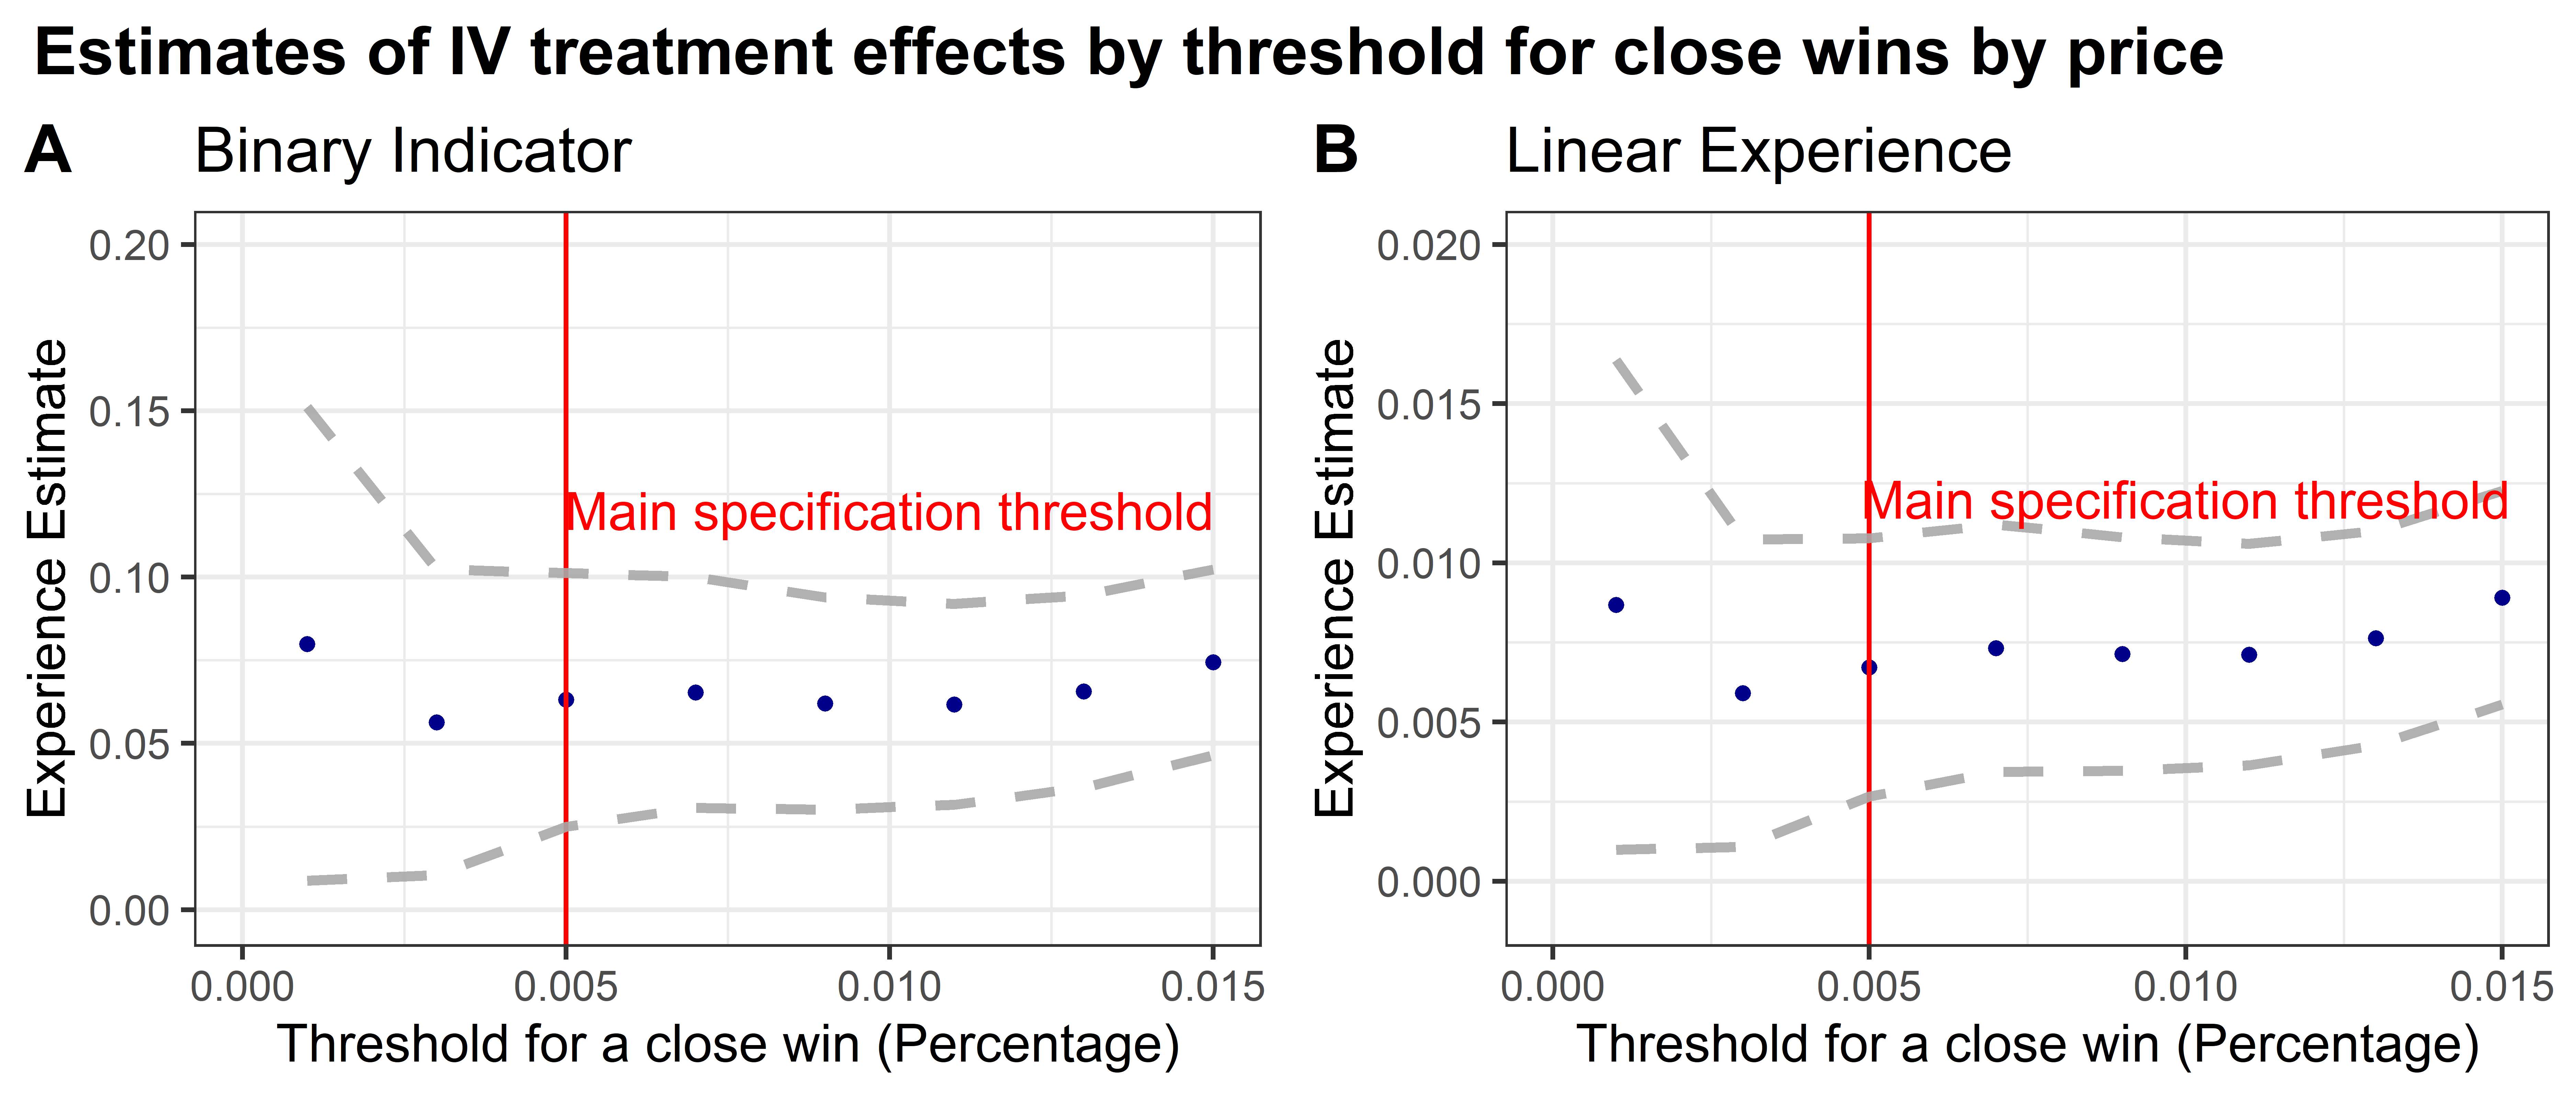
\includegraphics[scale=0.85]{robustness_threshold.png}
         \caption{Robustness analysis for threshold of close wins}
         \label{fig:close_wins_robust}

  \vskip 0.5mm
  {\justifying\footnotesize\underline{Note:} The plot shows the coefficient on experience as in the specification of Panel (5) of table \ref{tab:table_exp_1}, that is, the dependent variable is the share of contracts won in period $t$ and the dependent variable is linear experience, i.e. number of contracts won in period $(t-1)$, instrumented with close wins in period $(t-1)$. The $x$-axis shows how the coefficient varies with the threshold for what is considered a close win.\par}


     \end{figure}

%\chapter{Mechanisms}
Having established positive and significant treatment effects of  experience on outcomes in the market for public construction projects, we seek to investigate how does experience operate in practice to produce improved outcomes in the treated firms. Our objective is to provide evidence of some of the changes that might have taken place within the firm to produce a higher rate of success.

We start presenting the following working hypothesis regarding the effects of experience. Each details one way in which a firm might have experienced improvements that led to increased success in the market. Our analysis will be aimed at testing them with the data we have avalaible.

\begin{enumerate}
  \item{H1}: experience produces improvements in cost measures in the firm, keeping constant the type of project. This improvement in cost operates either via economies of scale, since after winning the project the firm is bigger than before; or via adjustments in the production function itself, for example, by changing the relative inputs to produce.
  \item{H2}: experience allows the firm to produce at a higher quality than before, constant the cost of the works. This improvement operates because the firm, having performed certain tasks once, is able to better predict potential problems. Note that in the bidding phase this could be reflected in a better proposals.
  \item{H3}: experience increases the pool of projects that a firm can perform. Experience can allow the firm to produce either bigger or more complex projects, due to increased human and organizational capital.
\end{enumerate}

We first investigate whether firms are more efficient by examining how do bids change on average with experience as treatment. Then, we study wether increased the technical possibilities of the firm.

\section{Bids and experience}
This section investigates whether experience causes improvements in cost measures for treated firms. We do this by examining how do firm's bids evolve after the firm has been treated, i.e. after it has more experience.

The relationship between bids and several firms characteristics has been investigated several times in the construction and economics literature.

The next section details briefly the data, empirical strategy and results, since most of the the empirical strategy and data is analogous to the analysis performed in the previous chapter.

\subsection{Data}

Our main data is the same as in the previous chapter, i.e a set of bids submitted by firms in auctions for public construction projects. However, instead of aggregating firm's experience and outcomes in time slices, our observations will be the bids themselves. We still employ aggregation to compute experience at each point in time for every firm.

Furthermore, we filter the first year in the data for our regression sample, since all firms have zero experience at this point and keeping it would introduce noise in the estimates do to treatments set to zero artificially. We do however employ all the avalaible years in the data to compute experience, as in the previous section.

Table \ref{} shows descriptive statistics of the bids employed in the analysis sample and of acecptance rates by the amount of experience.



\subsection{Empirical Strategy}
In this section, our main strategy is perform a regression of the form:

 Here, the outcome variable is a binary indicator which is 1 if the firm $i$ won the project $j$ at time $t$ and zero if not. Our treatment variable is experience, either in binary form $EXP>0$ or linear form $EXP$. We compute experience by summing all won up to $t$. Note that each row of our main dataset is an observation in the regression.
 %We employ an annualized form of experience to prevent overweighting the initial firms in the data.
Similarly as before, we have unobserved cost variables, specific to each firm, which might skew estimates upwards. The same argument employed in the previous chapter, regarding endogeneity of cost measures, can be applied in the case of equation.

We use the same strategy as before to produce consisten estimates, employing closely won bids to produce random variation in total experience. Table shows a comparison of contracts identified as close wins againts the rest of the sample. Note that there are very small modifications with respect to table \ref{}, given the extra filtering steps employed in this section. The parameters employed in each IV strategy are also the same as the previous section.

We perform four regressions. The first two are OLS regressions and the second two are IV regressions, employing closely won contracts to instrument total experience. For each type, we develop one regression where the treatment is the binarye of previous experience and the second is total past experience.

\subsection{Results}

Table \ref{tab:table_bids_1} presents our main results.

\input{C:/repos/learn-doing/thesis/tables/table_bids_1.txt}


%%%%%%%%%%%%%%%%%%%%%%%%%%%%%%%%%%%%%%%%%%%%%%%%%%%%%%%%%%%%%%%%%%%%%%%%%%%%%%%%%%%%%%%%%%%%%%%%%%%

\section{Quality and Experience}
In order to test hypothesis number two, in this section we study if experience treatments causes firms to submit higher quality proposals. We do this by employing a step in the auctioning process aimed at controlling some basic quality conditions of a proposals, namely, formal requirements and qualifications.

Note that quality is explicitly evaluated in many contracts by including an item in the awarding criteria labeled as "technical specifications" or just "quality of the proposal". Our estimation is that around \% include some measure of technical evaluation in the awarding criteria.  Ideally, we would test the hypothesis that experience improves the quality of a firm's proposals by employing the score that each firm obtained in the technical or quality item of the evaluation criteria of the project. However, since our data has not this item avalaible by firm, we employ an alternative strategy,which focuses on measuring quality across a different but related dimension: the formal acceptance rate of the proposals.

Recall that, for each auction, firm proposals are analyzed in two steps. The first step only examines if the proposal fulfills all the formal requirements in the process. Formal requirements include the inclusion of legal documents, submitting each of the technical documents asked for in the bidding documents, etc. In essence, the first stage verifies that all proposals can be evaluated at an equal footing and that minimum bidding legal requirements are fulfilled. Clearly, whether a proposal was accepted is a measure of its quality, albeit an imperfect one. Altough it leaves out a significant part of the variation that would be expected in proposal's qualities, it is nonetheless an interesting measure of quality because formal acceptance is a necessary condition to win a project.

Our research design, detailed below, will test whether experienced firms have a higher formal acceptance rate than unexperienced firms at the formal revision step of the procuurement process. To our knowledge, ity has not been studied in the previous literature factors infleuencing formal acceptance of bid proposals.

\subsection{Data}
We employ our bid dataset similarly as the previous section. Each observation is a bid submitted by a firm to an auction held by the government. Since we are analyzing the formal revision part of the auction, and not scoring itself, we think that on principle we could skip the filtering of contracts that do include experience as an awarding factor. However, due to possible self-selection, we will examine both possibilities. We again filter the first year of the data in our analysis sample to prevent confounding effects.

We show some descriptive statistics of acceptance rates in table and Figure \ref{fig:plot_acceptance_rates}. We can already see that the fraction of firms getting all proposals rejected decreases with more than one proposal, which could be either due to revealed preferences or to the effect of learning about formal requirements after the first completed bidding process.

\begin{figure}
  
\includegraphics[scale=0.50]{plot_acceptance_rates.png}
  \caption{Acceptance rate for proposals sent by firms to auctions for public construction project.}
  \label{fig:plot_acceptance_rates}
\end{figure}

We end up with a dataset where each observation is a bid submitted by a firm to an auction of a public construction project, which includes as variables of interest wether the proposal was formally accepted, the experience of the firm at the time of the auction (both regular, annualized and close wins), and several  auxiliary variables that characterize the contract itself.

\subsection{Empirical Strategy}
We test wether experience leads to a higher rate of formal proposal acceptance employing the following regression:

Here, is and indicator variable that equals 1 if the firms' $i$ proposal for contract $j$ at time $t$ was accepted and zero if it was not. $EXP$ is our treatment variable, both in binary and linear functional forms. $X_{j}$ is a set of contract-specific controls, which include year, region, and the government body in charge of the auction. We include the controls for the possibility that government units in different  geographical regions have different levels of stringency when evaluating proposals for similar projects.

We are less worried about endogeneity with unobserved cost factors since formal revision does not relate to economic aspects of the proposal. However, it is possible that there are different levels of baseline levels of proposal-makeing abilities among firms, so we repeat our usual instrumentation of experience with close wins.

We perform four regressions. The first two are OLS regressions and the second two are IV regressions, employing closely won contracts to instrument total experience. For each type, we develop one regression where the treatment is the binary of previous experience and the second is annualized past experience.

\subsection{Results}
\begin{figure}
  \includegraphics[scale=0.65]{plot_acceptance_results.png}
  \caption{Acceptance rate for proposals sent by firms to auctions for public construction project.}
  \label{fig:plot_acceptance_results}
\end{figure}

\input{C:/repos/learn-doing/thesis/tables/table_acceptance_1.txt}

%\chapter{Discussion}

In this chapter the results obtained are analyzed and the implications discussed.

\section{Experience and Outcomes}
Winning rates of firms with experience were successfully showed to be superior to the winning rates  of firms with no experience. We found a treatment effect of an increase of between seven and nine percentage points in winning rates for the treatment with any experience, and between .05 and 2 percentage points for every extra unit of experience. The magnitude of these effects seems to be relevant for the overall outcomes of a firm, since the mean rate of success when bidding is around 22\%. That means experience can render almost a 30\% improvement in future outcomes, measured as contracts won out of contracts bid for.

Our instrumental variables approaches to obtain consistent estimates were very different but rendered similar results. The first relied on close wins identified by close competition on price, while the second relied in finding contests between "similar firms", via a ranking algorithm. The advantage of the price strategy is that it is more interpretable, however, the conditions imposed were so stringent that the resulting "complier" sample was very small. The rank strategy is less interpretable, but theoretically it should control for any unobservable factor that influences firm's outcomes, not just cost advantages. The major weeakness of the rank strategy is the necessity of an adjustment period for newcomers, so ranks for first entrants (which are the most important ones) are less precise than those of firms which have been longer in the market. Additionally, having an additional set of parameter (points awarded for win and lose) can make the strategy less  robust.

Interestingly, the IV strategies rendered almost always higher estimates than the OLS, when the original hypothesis was that an upwards bias would be found. Two points can be mentioned to explain this. First, the experience measure (contracts won, in any of its forms) is a noisy measure of experience, since actual learning or improvements depends highly on the size of the contract, type of project, etc. Then, there is an attenuation effect in the OLS estimates.

The second possibility is that there is a selection effect which takes out firms from the market when they are unable to gain experience. In principle, the effect of experience on entry and exit is uncertain. If the environment is too hostile, for example, firms encounter a high level of bureaucracy in thei contracts, experience might induce exit. However, if firms perceive returns to experience, we should see increased exit among non-experienced firms. In the latter case, the treatment effect of experience underestimates the true returns to experience, since firms in the market survive precisely because of the it.  The OLS estimates underestimate the true effect of experience because we do not observe outcomes for firms that were unable to gain experience and had to abandon the market following defeats in the auctions. We briefly show in plot how exits disaggregated in terms of \% of firms that exit with and withoutt experience per year.

A limitation of the analysis is that it is only able to identify the Local Average Treatment Effect, which in the current context is interpreted as the treatment effect for those firms that can only acquire experience through a close win. Given our restrictive instruments' definition, this feature of the distribution of the causal effects is only applicable to a small part of our observations (between 2\% and 15\%, depending on the instrument). However, this is arguably the most important subsample, because among them are possibly firms that would achieve significant improvements after acquiring experience. Also, this discussion could show more evidence as to why we obtain higher IV than OLS estimates. Given the choice of the instrument, a firm that would only win in a close win should not have an absolute advantages in the market already, so it has more room to grow.

The comparison of estimates for the treatment effect of experience between contracts that explicitly rewarded experience and those that did not (the main reslts) is relevant because it shows that the implicit effect of experience on outcomes is at least in the same order of magnitude as the explicit effect. The explicit estimate of the treatment effect of any experience was around seven percentage points, while for contracts that did not require it was seven percentage points . Given this, policymakers might prefer to only employ experience as a prequalification method, since it seems to largely operate in the case of no explicit reward for experience.

We found low $R^2$ in our regressions which shows that there is considerable heterogeneity in the outcomes. This can be attributed to the fact that we employed minimal types of controls in the regressions and wide array of types, locations, buyers and sellers. An alternative strategy would have been to i) add more controls or ii) consider a more restrictive market. Option i) was not employed because the sample is unbalanced in many ways and also because we do not have detailed contract description variables that could have been employed to control. Option ii) could be used to obtain a more precise estimate in a clearly defined subsample, like contracts that need prequalification in the Ministry of Housing or Public Works. However, for these two government units the information was either incomplete or there was not a clear way to distinguish more "restricted" contracts beyond size.

\section{Operational Mechanisms of Experience}

The mechanisms section's objective was to test hypothesis about the improvements caused by experience in treated firms. Two possibilities were examined: improvements in cost measures, measured by the level of standarized bids submitted; and  quality levels, measured by the rate of acceptance of offers in a stage of the procurement process that verifies fulfillment of formal and/or technical requirements in proposals.

Firstly, the hypothesis that experience causes reduction in cost measures was tested. It was found that bids of firms with more than zero experience were between three and four percentage points lower than those that did not have any. The average difference between lowest and second lowest firms is around seven percentage points, so the impact can be significant if there is a binary reward to the lowest bid submitted. In this investigation, unlike most of our tests, we found linear experience to not have a significant coefficient. This might because this analysis employed total experience, with no adaptations such as annualizing or considering shorter periods. Given that at the last observations we have firms with very high measures of experiences (>100 contracts) it is expected that due to diminishing returns a linear return on experience is not the best choice.

Is an improvement of three percentage points truly useful to win more contracts? The results on lower bid amounts were significant, but it could be argued that the wide amount of factors employed to award projects render the effect negligible. However, a quick regression of the winning outcome (0-1) of the auction (for each firm that submitted a proposal) on standarized bids, with the usual fixed effects (see Appendix for details) shows that for every less percentage point on bid amounts, winning probability increase by around . Thus, there at least correlation between lowered bid submitted and winning probability.

The result that first entrants bid more aggresively than firms with more than one year in the market was in line with previous literature results. Notably, the net effect of experience and first entry shows that an experienced firm still submits lower bids on average than first entrants.

The second hypothesis examined was that experience improves the quality of the proposals that a firm submits for auctions. The acceptance rate of proposals in the formal check stage of the procurement process was employed as a quality measure. We found that firms with stricly positive experience have acceptance rates that are around ten percentage points higher than firms with no experience. This effect is relevant considering that the average rate of acceptance is around 80\%, so the effect of experience drives acceptance rates close to 90\%.

It could be argued that the effect observed corresponds only to an adaptation experienced naturally after participating in the first "trial" auctions and that it only comes from bidding instead of experience. Howevever, the analogous treatment effect of $bidding \ experience$ on outcomes is only percentage points (details on the Appendix). While there seems to be a component of the effect realted to "knowing the market", the effect of experience goes above and beyond this.

A remark should be made regarding the assumption that improved acceptance rates are related to improved quality. The improved quality identified in the result should be interpreted narrowly here as a better consideration of formal requirements in the proposal. A reasonable assumption is that all quality aspects of a bid are correlated and then that this relates to overall improvements in quality measures for the firm.

Overall, we mostly discussed costs measures, bids and quality as evolving due to within-firm changes. In this context, increased winning rates and improved acceptance rates are "positive". However, a part of these outcomes could be related to rent-seeking and capture of the market, by knowing "tricks" that inexperienced firms do not, or even corruption. The existence of legal rules  and the employment of a digital platforms constructed to prevent communication or knowledge of biders before the awarding decision should diminish the opportunity for these types of situations. Still, we cannot completely rule them out.

\section{Data and Others Considerations}
A contribution of this project was to employ a comprehensive set of data regarding public purchases with ten years of public purchases. The data contained a great deal of useful and detailed variables, which were key for the investigation and are rarely avalaible in other similar investigations about bidding behaviour. The most important advantage of the dataset is that it covered almost all government bodies, which allows to construct a measure of public experience that we believe is very close to the actual level of experience in open call for proposal auctions. Investigations conducted previously in the literature tend to rely on markets much more restricted in scope, considering for example in the U.S case usually road projects from the Department on Transportation.

There are still ways to improve the data. It is hard to store sytematically the scores of a proposal in every item, since they differ among contracts. Nonetheless, some elements, like experience, price and quantity items could be made standard fields and stored due to their prevalence. The most difficult part of data collection was to gather the data for the awarding criteria, since it is unstructured (not in a database) and gathering it required to employ a (capped) API and manually programming a scraper to crawl the required information. Fortunately, the awarding criteria was usually stored similarly in the relevant webpage for every contract (the difficult part is knowing the URL of the webpage). Still, we had around 10\%-15\% of contracts with missing data on these fields, which had to be dropped from outcome computation.

Another regrettable omission of the data is the lack of comprehensive data for the Ministry of Public Projects. While on absolute numbers the contracts of this government unit are less to the ones of municipalities, for example, because of their complexity and size they are expected to have high returns to experience and of more interest. This organism started publishing their data comprehensively only since 2017, so before that year the data is incomplete.

\section{Implications for the market}
The magnitude of the effects found for experience could work as an entry barrier for new entrants to public construction projects. However, the econometrical interpretation of our treatment effects allows only us to say that firms that get in the market because of "random" wins improve in their outcomes. In that sense, the results points towards experience as an entry barrier for firms without strong comparative advantages in the market \textit{ex ante}.

The effect on the competitveness on the market (only considering the treatment found) is then to limit the possibility of surgence of "bad" firms which would become "good" with some experience. While this would be probably an undesirable feature in a private market, it could be argued that public markets should be focused on procuring goods as efficiently as possible. Then, depending on the tolerance to the distortion of preventing some firms to develop in the market, a policymaker might not be troubled by the results observed.

A possible effect suggested by the results is double-counting when considering experience in the award criteria. As it was seen, almost 60\% of the contracts include experience in the awarding criteria. However, it was also seen that more experience contractors already display qualities taht make them more likely to be selected as contractors, like lower cost measures and better proposals. Then, from a competitve perspective, it could be better to rise technical or economical requirements to award the project but diminish the experience requirement (which as was discussed is also a noisy measure of skill). If experience is truly a desirable propert, we expect its effects to manifest in other aspects of the proposal that will make it more likely to be awarded the project anyways.

%This could be a desirable outcome, since we have shown that more experienced firms submit proposals with higher rates of acceptance and more economical.

\chapter{Conclusion}
This paper's objective was to understand the treatment effect of experience on outcomes in the market of public construction projects. The investigation analyzed around 150,000 bids from contracts to compare the rate at which firms with and without experience win contracts in the future. The investigation also aanalyzed possible mechanisms that would explain improved outcomes for firms with experience: a disminution of firm's cost measures, as measured by standarized bids submitted; and improved proposal quality, as measured by the acceptance rate of firm's proposals in a stage of the procurement process where formal requirements are processed.

The main empirical strategy was to slice the dataset in different points in time and compare outcomes for the different levels of the treatment measures. Also, close wins were employed as source of random variation to instrument total wins, since experience is probably endogenous in the market. Close wins were defined employing a price strategy, where close wins are the ones where bids were close and price was a major awarding factor; and rank strategy, where a ranking was constructed for every firm and thus identify contests among similar contracts. Altough both were second-best strategies employed due to the lack of proposal's score variables, both alternatives, along with most of an extensive set of robustness results, yielded similar outcomes.

The work could be complemented in the future by a general model of bidding in the public sector. The heterogeneity of outcomes that we found shows that this effort would require to improve in the characterization of both units and contracts to yield detailed results at the firm level. On a separate field, the variables constructed would be also useful to construct a machine learning approach to detect suspicious awarding decisions.


%\appendix
%\chapter{Appendix}
\section{Rank Regressions}
\label{section:appendix_rank}
The following regressions have as dependent variable experience and as independent variable close experience, which is our instrument in the main results section. Table \ref{tab:table_F_main_exp2} shows the results for the first measure of experience (rolling), while Table \ref{tab:table_F_main_exp2} shows the results for the second measure of experience (annualized cumulative).
\input{C:/repos/learn-doing/thesis/tables/table_F_main_exp1.txt}

\input{C:/repos/learn-doing/thesis/tables/table_F_main_exp2.txt}
\clearpage
\section{Additional Sample Characterization}
This section expands on the sample characterization of the Data chapter. Regional and market participants descriptions are included in the form of tables or graphs.

\subsection{Regional Representation}
\input{C:/repos/learn-doing/thesis/tables/sampleregion.txt}
\clearpage

\subsection{Top Market Participants}
\input{C:/repos/learn-doing/thesis/tables/topgov.txt}
\small
\input{C:/repos/learn-doing/thesis/tables/topfirms.txt}
\clearpage


\section{Bids and Winning Probability}
This section explores the relationship between bids and winning probability. We develop two simple regressions of the form:
\begin{equation}
  \label{eqn:helpbids}
INDWIN_{ij}  = \alpha +BID_{ij}+  FIRSTYEAR_{ij}+X_j\varepsilon_{ij}
\end{equation}
Where $INDWIN$ is an indicator for winning the firm $i$ submitting a winning bid for contract $j$, $BID$ is a standarized bid, and $X_j$ are controls for the contract. In the first specification, $X_j$ are just fixed effects for Year and Region. In the second specification, we employ per-contract Fixed Effects, which means that we identify the parameter of interest through the variation in bids and outcomes for the participants in the same auction. The second specification omits the intercept as well.

Our sample consists in contracts for which i) there were two or more valid participants and ii) had a winner chosen. This renders 29,608 observations. The regressions are at the firm-bid level.

Results are shown in Table \ref{tab:table_bids_help}. Notably, the results imply that a three percentage point decrease in the standarize bid is correlated with an increase of ten percentage points in winning probability. Given that previous discussions showed that price is an awarding component in most contracts, there seems to be enough basis to establish a causal nexus between submitting lower bids and winning contracts, altough there is still much uncertainty about the actual magnitude. For similar  example, probably all firms' measures of quality are probably correlated, so we cannot attribute the win to smaller bids alone.

\input{C:/repos/learn-doing/thesis/tables/table_bids_help.txt}

\clearpage
\section{ELO algorithm : theory and implementation}
\label{section:eloappendix}
\subsection{Introduction}\footnote{This section is based on Arpad Elo's book introduction to the Elo system in \citep{elo1978rating}}
The Elo Ranking is a system to place players in a numerical rating scale, in which differences among players can be converted into scoring or winning probabilities. Similarly, scoring percentages (over time or competitions) can be converted into ranking differences. Ratings in the Elo system are points in a scale which, for historical reasons, has been chosen to have its midpoint at 2000. However, the importance is on difference of ratings rather than in absolute number, since a Elo ranking is only valid within a specific pool of players.

The first basic principle of the Elo system is that performances from an individual are normally distributed, when evaluated on an appropriate scale. Let the expectancy score be the expected number of points that a player is expected to win, out of the total possible, in a match or matches. According to Elo, the percentage expectancy score for a player is a function of the difference in rating with the opponent. For example, a player one standard deviation in ranking above another has an approximate  percentage expectancy score. This follows from a standard computation of the probability that a draw from a random variable of mean $\mu_1$ and standard deviation $\sigma$ is higher than a random variable of mean $\mu_2$ and standard deviation $\sigma$ as well.

The performance of a player is evaluated on the basis of how do his or her actual performance compare to the expected score, both of his own and his opponents. The \textit{Perfomance Rating} is a measure of performance evaluated over a number of encounters which combines the average rating of the competition and the percent score achieved. A more stable measure over time is the \textit{Player rating} which ought to vary less than the performance rating. In the context of chess, where it was developed, a performance rating would be obtained for a chess tournament, while the rating of the player would be his overall ranking. The player rating can be updated periodically through Performance Ratings as follows.

Over intervals, rankings for players can be calculated using the Performance Rating formula:
\begin{equation}
  R_p=R_c+D_p
  \label{ratingdiscrete}
\end{equation}
Where $R_p$ is the performance rating, $R_c$ is the average rating and $D_p$ is the difference based on the percentage score $P$, which is obtained from the curve or table. This formula can be employed to update rankings over periods of time. However, to maintain a continuous ranking (i.e. at every point in time), the following formula is used:
\begin{equation}
  R_n=R_0 + K(W-W-_e)
  \label{ratingcontinuous}
\end{equation}
Where $R_n$ is the rating after the event, $R_0$ is the rating pre-event, $K$ is the rating point value of a single game score, $W$ is the actual game score, and $W_e$ is the expected game score based on $R_0$. The parameter $K$ adjusts the relative weight of newer and older performances. A higher $K$ gives a higher weight to newer performances, and vice versa.

\subsection{Current Implementation}
The algorithm employed in the current investigation is a modified  Elo system suited for multiplayer games with variable player numbers. The implementation used is contained the function $elom$ of the R package \textit{PlayerRatings}, which implements several types of ranking algorithms \citep{stephenson2020package}. The adaptation of the canonical Elo algorithm to allow for a variable number of (multiple) players requires to i) implement a computation of expected scores that considers the wider range of competitors, and ii) change the way points are awarded and substracted depending on the actual number of players for a game.

For algorithmic purposes, we consider a win as being awarded a contract and a lose as bidding for but not winning a specific contract. All losing players are considered "tied" in their loss, so base points substracted are the same. However, actual points substracted might differ depending on the expected score, as shown in Equation \ref{eqn:ratingadjust}.

The initial rating of a player was chosen to be 1,500. Also, since an adaptation time is needed to construct a reliable average rank, for all the analysis employing the ranking measure the first year of the data is discarded (after constructing the ranks). The documentation of the implemented algorithm recommends to make it so the net number of awarded points after a game is zero. Although keeping this recommendation and keeping the same number of points for every contest constant is impossible, we choose awarded and subtracted points such that this is true for the average contract\footnote{It would be possible the assign scores based on number of players in the contest. However, for parsimony and ease of validation purposes we take the approach to fix constant the scores.}.

To construct the ranking, the following computation steps were performed:
\begin{enumerate}[itemsep=1pt]
  \item The data was filtered to contain only contracts for which there were two or more opponents and which had a winner contractor. This renders approx. 29,000 contracts.
  \item The relevant competition datasets were constructed. In these datasets, every observation is an auction with two or more players. Columns are participants. The columns contain the names of the participants in the auction. A similar dataset contains the outcomes for each player participating.
  \item The ranking algorithm was run with the match history as the key input.
\end{enumerate}
Results consists in a ranking for every firm at every contract in the sample constructed in point 2. For interpretation purposes, rankings for contracts filtered out from the main sample are filled by i) getting the ranking of the closest past contract which performed a ranking update or ii) imputing the base rank, for contractors who did not have any contracts with ranking updates. The latter can happen if a contractor bids only in contracts where he is the only bidder \footnote{Note that for instrument construction, any contract with an imputed ranking cannot, by definition, be labeled as a close win, since this requires two or more players and a winner as a necessary condition}.

Later, in the main estimation step, the rankings are employed to identify close wins, as described in the empirical strategy section. Note that the algorithm itself employs the assumption that, for (two) equally ranked opponents, winning chances are 50 - 50. Wins against close opponents are thus attributed in both schemes mainly to random factors.

\subsection{Analysis of algorithm results}
In this section we describe some of the results to validate and interpret the rankings obtained. Figure \ref{fig:rankings_nums} shows the progression of ranks over the history of firms. Every panel is the distribution of firms at a point in their bidding history. For example, panel two shows the distribution of ranks between firms who are bidding for the second time. Note that ranks split in two after the first bidding by the win or a lose. Successive biddings "fill in" the gaps. Given that points awarded for wins are more than points substracted by loses, the distributions are right-skewed.

\begin{figure}[H]
\centering
  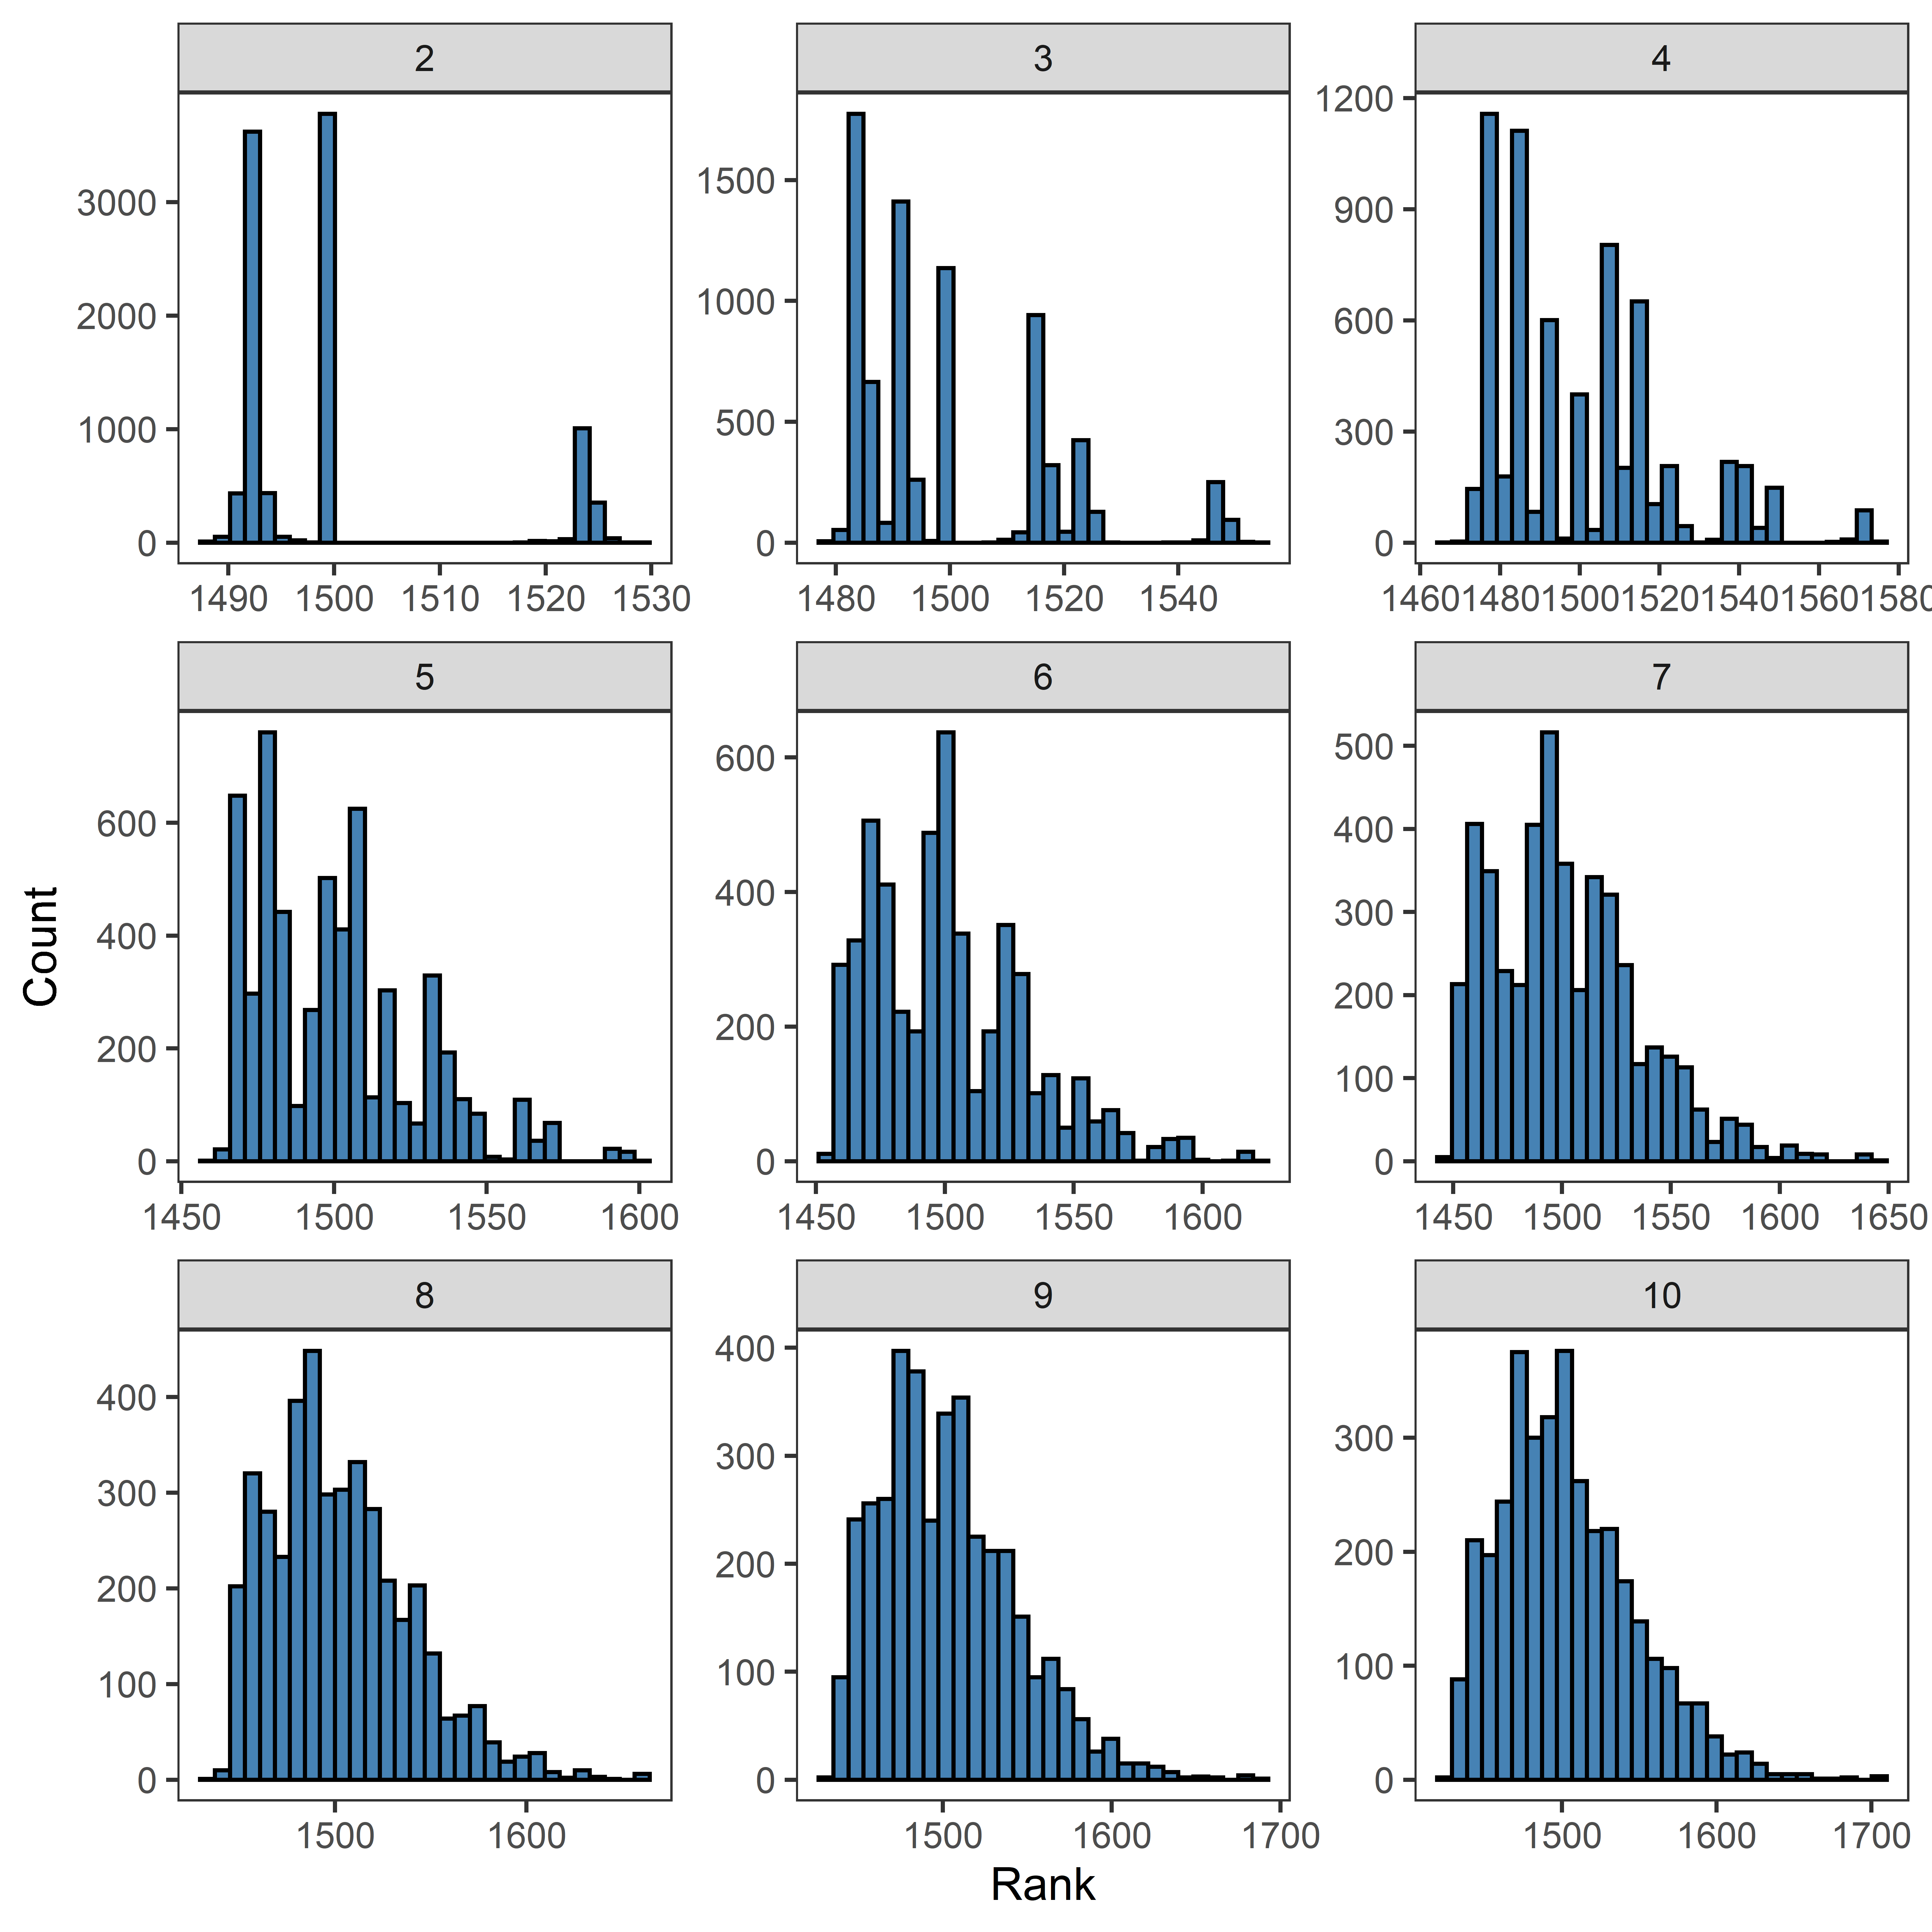
\includegraphics[scale=0.9]{rankings_nums}
  \caption{Rank progression over firm's bidding history \\ \footnotesize \underline{Note}: each panel contains the firms bidding for their $i$-th contract. The graph only displays the ranks for the first 10 bidding events. Ranks displayed are ranks $previous$ to the contract, i.e. they are not adjusted by the outcome of the i-th bidding event.}
  \label{fig:rankings_nums}
\end{figure}

The progression of rankings over time is further illustrat ed with two firms which end higher and lower respectively in ranking than their starting points at 1,500. We call the first firm "A" and the second firm "B".  The next tables show the contracts participated in, the ranking at each contract, the average ranking of opponents, the result of the bidding (i.e. win or lose) and the net effect of the "game" of the firm's ranking (measured in points). Table \ref{tab:rank_example_1} shows a firm which won all but its last contracts. While all winning contracts resulted in points added to ranking, the first wins rendered more points, as the advantage of the firm was lower. Table \ref{tab:rank_example_2} shows firm B, which mostly experienced defeats. Note that points substracted by losing are less than the ones granted for winning, so the ranking still remains close to 1,500. Also, this firm faced similar opponents, as measured by the similar average ranks.

\input{C:/repos/learn-doing/thesis/tables/rank_example_1.txt}

\input{C:/repos/learn-doing/thesis/tables/rank_example_2.txt}


%\chapter{Tables}

\begin{table}
\caption{Armadillos}
\label{arm:table}
\begin{center}
\begin{tabular}{||l|l||}\hline
Armadillos & are \\\hline
our	   & friends \\\hline
\end{tabular}
\end{center}
\end{table}

\clearpage
\newpage

%\chapter{Figures}

\vspace*{-3in}

\begin{figure}
\vspace{2.4in}
\caption{Armadillo slaying lawyer.}
\label{arm:fig1}
\end{figure}
\clearpage
\newpage

\begin{figure}
\vspace{2.4in}
\caption{Armadillo eradicating national debt.}
\label{arm:fig2}
\end{figure}
\clearpage
\newpage


\printbibliography
\end{document}
